\documentclass[twoside]{book}

% Packages required by doxygen
\usepackage{fixltx2e}
\usepackage{calc}
\usepackage{doxygen}
\usepackage{graphicx}
\usepackage[utf8]{inputenc}
\usepackage{makeidx}
\usepackage{multicol}
\usepackage{multirow}
\PassOptionsToPackage{warn}{textcomp}
\usepackage{textcomp}
\usepackage[nointegrals]{wasysym}
\usepackage[table]{xcolor}

% Font selection
\usepackage[T1]{fontenc}
\usepackage{mathptmx}
\usepackage[scaled=.90]{helvet}
\usepackage{courier}
\usepackage{amssymb}
\usepackage{sectsty}
\renewcommand{\familydefault}{\sfdefault}
\allsectionsfont{%
  \fontseries{bc}\selectfont%
  \color{darkgray}%
}
\renewcommand{\DoxyLabelFont}{%
  \fontseries{bc}\selectfont%
  \color{darkgray}%
}
\newcommand{\+}{\discretionary{\mbox{\scriptsize$\hookleftarrow$}}{}{}}

% Page & text layout
\usepackage{geometry}
\geometry{%
  a4paper,%
  top=2.5cm,%
  bottom=2.5cm,%
  left=2.5cm,%
  right=2.5cm%
}
\tolerance=750
\hfuzz=15pt
\hbadness=750
\setlength{\emergencystretch}{15pt}
\setlength{\parindent}{0cm}
\setlength{\parskip}{0.2cm}
\makeatletter
\renewcommand{\paragraph}{%
  \@startsection{paragraph}{4}{0ex}{-1.0ex}{1.0ex}{%
    \normalfont\normalsize\bfseries\SS@parafont%
  }%
}
\renewcommand{\subparagraph}{%
  \@startsection{subparagraph}{5}{0ex}{-1.0ex}{1.0ex}{%
    \normalfont\normalsize\bfseries\SS@subparafont%
  }%
}
\makeatother

% Headers & footers
\usepackage{fancyhdr}
\pagestyle{fancyplain}
\fancyhead[LE]{\fancyplain{}{\bfseries\thepage}}
\fancyhead[CE]{\fancyplain{}{}}
\fancyhead[RE]{\fancyplain{}{\bfseries\leftmark}}
\fancyhead[LO]{\fancyplain{}{\bfseries\rightmark}}
\fancyhead[CO]{\fancyplain{}{}}
\fancyhead[RO]{\fancyplain{}{\bfseries\thepage}}
\fancyfoot[LE]{\fancyplain{}{}}
\fancyfoot[CE]{\fancyplain{}{}}
\fancyfoot[RE]{\fancyplain{}{\bfseries\scriptsize Generated on Sat Nov 21 2015 21\+:25\+:48 for Stack\+Machine\+Dual\+Operand by Doxygen }}
\fancyfoot[LO]{\fancyplain{}{\bfseries\scriptsize Generated on Sat Nov 21 2015 21\+:25\+:48 for Stack\+Machine\+Dual\+Operand by Doxygen }}
\fancyfoot[CO]{\fancyplain{}{}}
\fancyfoot[RO]{\fancyplain{}{}}
\renewcommand{\footrulewidth}{0.4pt}
\renewcommand{\chaptermark}[1]{%
  \markboth{#1}{}%
}
\renewcommand{\sectionmark}[1]{%
  \markright{\thesection\ #1}%
}

% Indices & bibliography
\usepackage{natbib}
\usepackage[titles]{tocloft}
\setcounter{tocdepth}{3}
\setcounter{secnumdepth}{5}
\makeindex

% Hyperlinks (required, but should be loaded last)
\usepackage{ifpdf}
\ifpdf
  \usepackage[pdftex,pagebackref=true]{hyperref}
\else
  \usepackage[ps2pdf,pagebackref=true]{hyperref}
\fi
\hypersetup{%
  colorlinks=true,%
  linkcolor=blue,%
  citecolor=blue,%
  unicode%
}

% Custom commands
\newcommand{\clearemptydoublepage}{%
  \newpage{\pagestyle{empty}\cleardoublepage}%
}


%===== C O N T E N T S =====

\begin{document}

% Titlepage & ToC
\hypersetup{pageanchor=false,
             bookmarks=true,
             bookmarksnumbered=true,
             pdfencoding=unicode
            }
\pagenumbering{roman}
\begin{titlepage}
\vspace*{7cm}
\begin{center}%
{\Large Stack\+Machine\+Dual\+Operand \\[1ex]\large 1.\+0 }\\
\vspace*{1cm}
{\large Generated by Doxygen 1.8.8}\\
\vspace*{0.5cm}
{\small Sat Nov 21 2015 21:25:48}\\
\end{center}
\end{titlepage}
\clearemptydoublepage
\tableofcontents
\clearemptydoublepage
\pagenumbering{arabic}
\hypersetup{pageanchor=true}

%--- Begin generated contents ---
\chapter{Class Index}
\section{Class List}
Here are the classes, structs, unions and interfaces with brief descriptions\+:\begin{DoxyCompactList}
\item\contentsline{section}{\hyperlink{classAlu}{Alu} \\*Unidade Lógico Aritmética }{\pageref{classAlu}}{}
\item\contentsline{section}{\hyperlink{classDataStack}{Data\+Stack} \\*Pilha de dados }{\pageref{classDataStack}}{}
\item\contentsline{section}{\hyperlink{classDSController}{D\+S\+Controller} \\*Controlador da pilha de dados }{\pageref{classDSController}}{}
\item\contentsline{section}{\hyperlink{classFetch}{Fetch} \\*Interface da R\+O\+M com o resto do sistema }{\pageref{classFetch}}{}
\item\contentsline{section}{\hyperlink{classFileHandler}{File\+Handler} \\*Gerenciador de arquivos }{\pageref{classFileHandler}}{}
\item\contentsline{section}{\hyperlink{classRam}{Ram} \\*Random Access Memory }{\pageref{classRam}}{}
\item\contentsline{section}{\hyperlink{classRom}{Rom} \\*Read-\/\+Only Memory }{\pageref{classRom}}{}
\item\contentsline{section}{\hyperlink{classStack}{Stack} \\*Pilha de retorno }{\pageref{classStack}}{}
\end{DoxyCompactList}

\chapter{File Index}
\section{File List}
Here is a list of all documented files with brief descriptions\+:\begin{DoxyCompactList}
\item\contentsline{section}{\hyperlink{Alu_8cpp}{Alu.\+cpp} }{\pageref{Alu_8cpp}}{}
\item\contentsline{section}{\hyperlink{Alu_8h}{Alu.\+h} }{\pageref{Alu_8h}}{}
\item\contentsline{section}{\hyperlink{DataStack_8cpp}{Data\+Stack.\+cpp} }{\pageref{DataStack_8cpp}}{}
\item\contentsline{section}{\hyperlink{DataStack_8h}{Data\+Stack.\+h} }{\pageref{DataStack_8h}}{}
\item\contentsline{section}{\hyperlink{Defines_8h}{Defines.\+h} \\*Definição de valores fixos do sistema }{\pageref{Defines_8h}}{}
\item\contentsline{section}{\hyperlink{Fetch_8cpp}{Fetch.\+cpp} }{\pageref{Fetch_8cpp}}{}
\item\contentsline{section}{\hyperlink{Fetch_8h}{Fetch.\+h} }{\pageref{Fetch_8h}}{}
\item\contentsline{section}{\hyperlink{FileHandler_8cpp}{File\+Handler.\+cpp} }{\pageref{FileHandler_8cpp}}{}
\item\contentsline{section}{\hyperlink{Main_8cpp}{Main.\+cpp} \\*Método main }{\pageref{Main_8cpp}}{}
\item\contentsline{section}{\hyperlink{Ram_8cpp}{Ram.\+cpp} }{\pageref{Ram_8cpp}}{}
\item\contentsline{section}{\hyperlink{Ram_8h}{Ram.\+h} }{\pageref{Ram_8h}}{}
\item\contentsline{section}{\hyperlink{ReturnStack_8cpp}{Return\+Stack.\+cpp} }{\pageref{ReturnStack_8cpp}}{}
\item\contentsline{section}{\hyperlink{ReturnStack_8h}{Return\+Stack.\+h} }{\pageref{ReturnStack_8h}}{}
\item\contentsline{section}{\hyperlink{Rom_8cpp}{Rom.\+cpp} }{\pageref{Rom_8cpp}}{}
\item\contentsline{section}{\hyperlink{Rom_8h}{Rom.\+h} }{\pageref{Rom_8h}}{}
\end{DoxyCompactList}

\chapter{Class Documentation}
\hypertarget{classAlu}{\section{Alu Class Reference}
\label{classAlu}\index{Alu@{Alu}}
}


Unidade Lógico Aritmética.  




{\ttfamily \#include $<$Alu.\+h$>$}



Inherits sc\+\_\+module.

\subsection*{Public Member Functions}
\begin{DoxyCompactItemize}
\item 
void \hyperlink{classAlu_a7a60dcc8e76a08c1cd20597f84cbd321}{set\+Buffers\+D\+S} (int buf\mbox{[}4\mbox{]})
\item 
void \hyperlink{classAlu_ab413ef21248de9a39c543d0fd1c233cb}{set\+Buffers\+R\+S} (int buf\mbox{[}4\mbox{]})
\item 
void \hyperlink{classAlu_ab3a692120ec7c7a1b7625b8f601272a6}{set\+P\+C} (int $\ast$pc)
\item 
void \hyperlink{classAlu_a68e91decd645362078515555cde833e7}{set\+D\+S\+P} (int $\ast$dsp)
\item 
void \hyperlink{classAlu_aa507af8006a2862c7b17a3d637ce38de}{set\+R\+S\+P} (int $\ast$rsp)
\item 
void \hyperlink{classAlu_af34256a02a7be19a7d60a910db157210}{set\+Sizes} (int $\ast$dss, int $\ast$rss)
\item 
virtual void \hyperlink{classAlu_ad8e186aac3201dc8a26cc61d7a90c5d2}{b\+\_\+transport\+\_\+\+Fet} (tlm\+::tlm\+\_\+generic\+\_\+payload \&trans, sc\+\_\+time \&delay)
\item 
\hyperlink{classAlu_aab26dc9ed3cb4bdd1d13206f19a00552}{$\sim$\+Alu} ()
\end{DoxyCompactItemize}
\subsection*{Private Member Functions}
\begin{DoxyCompactItemize}
\item 
void \hyperlink{classAlu_a3fabfe3b33df17581f8bc85de9eddeea}{compute} ()
\item 
void \hyperlink{classAlu_adf5731c0d59b22371ad9403afaaacff4}{write\+D\+S} (int adr, int op)
\item 
void \hyperlink{classAlu_a5ae5ca371b090c716236619f2d63fd74}{write\+R\+S} (int adr, int op)
\item 
void \hyperlink{classAlu_a2ab3afd02491a49f20c141c694c2ecbe}{write\+R\+S} (int adr, tlm\+::tlm\+\_\+command cmd)
\item 
void \hyperlink{classAlu_ad82f3646bf0843beabf5d0ee18d6e273}{write\+D\+S} (int adr, tlm\+::tlm\+\_\+command cmd)
\item 
void \hyperlink{classAlu_aee7f8876c2ebe00f52e3bb55d8f86b73}{write\+R\+A\+M} (int addr, int op)
\item 
int \hyperlink{classAlu_a059b74a69d274885568cfbb2e31fc603}{read\+R\+A\+M} (int addr)
\item 
int \hyperlink{classAlu_a05a5eb6c972a875195498e91f5418706}{pick\+Source} (int op)
\item 
void \hyperlink{classAlu_a39455b035f0298a546de937f9ab21426}{store\+Source} (int op, int data)
\end{DoxyCompactItemize}
\subsection*{Private Attributes}
\begin{DoxyCompactItemize}
\item 
sc\+\_\+int$<$ \hyperlink{Defines_8h_af087b76f9707be9d3b43ba0c782c31c3}{D\+A\+T\+A\+\_\+\+W\+I\+D\+T\+H} $>$ \hyperlink{classAlu_a307709e37d80c03970b0165d29dfb4c4}{instruction}
\item 
int $\ast$ \hyperlink{classAlu_afc87096d954e9091302d7c1854a910e1}{P\+C}
\item 
int $\ast$ \hyperlink{classAlu_a259ee7ef49be47158d26c8c3a0ae1feb}{buffers\+D\+S}
\item 
int $\ast$ \hyperlink{classAlu_a4b54db20f10aed5d7d70378b5c9a77fd}{buffers\+R\+S}
\item 
int $\ast$ \hyperlink{classAlu_aea20506a48d2027cd27a0c2aec32a4c7}{D\+S\+P}
\item 
int $\ast$ \hyperlink{classAlu_ad6e5dacce0eecd38c727b6cc5877d05c}{R\+S\+P}
\item 
int $\ast$ \hyperlink{classAlu_ab0be93bc681fe3791cbd8a815d018a89}{D\+S\+S}
\item 
int $\ast$ \hyperlink{classAlu_abd81e60239f46572212450b326f2261d}{R\+S\+S}
\end{DoxyCompactItemize}


\subsection{Detailed Description}
Unidade Lógico Aritmética. 

Módulo responsável pela computação dos valores carregados das pilhas e por alocar o resultado na pilha de destino ou em memória.

\begin{DoxyAuthor}{Author}
Gerson Miguel Beckenkamp 
\end{DoxyAuthor}
\begin{DoxyDate}{Date}
2015/09/05 14\+:16\+:20 
\end{DoxyDate}


Definition at line 35 of file Alu.\+h.



\subsection{Constructor \& Destructor Documentation}
\hypertarget{classAlu_aab26dc9ed3cb4bdd1d13206f19a00552}{\index{Alu@{Alu}!````~Alu@{$\sim$\+Alu}}
\index{````~Alu@{$\sim$\+Alu}!Alu@{Alu}}
\subsubsection[{$\sim$\+Alu}]{\setlength{\rightskip}{0pt plus 5cm}Alu\+::$\sim$\+Alu (
\begin{DoxyParamCaption}
{}
\end{DoxyParamCaption}
)}}\label{classAlu_aab26dc9ed3cb4bdd1d13206f19a00552}
Destrutor do módulo 

Definition at line 1430 of file Alu.\+cpp.



\subsection{Member Function Documentation}
\hypertarget{classAlu_ad8e186aac3201dc8a26cc61d7a90c5d2}{\index{Alu@{Alu}!b\+\_\+transport\+\_\+\+Fet@{b\+\_\+transport\+\_\+\+Fet}}
\index{b\+\_\+transport\+\_\+\+Fet@{b\+\_\+transport\+\_\+\+Fet}!Alu@{Alu}}
\subsubsection[{b\+\_\+transport\+\_\+\+Fet}]{\setlength{\rightskip}{0pt plus 5cm}void Alu\+::b\+\_\+transport\+\_\+\+Fet (
\begin{DoxyParamCaption}
\item[{tlm\+::tlm\+\_\+generic\+\_\+payload \&}]{trans, }
\item[{sc\+\_\+time \&}]{delay}
\end{DoxyParamCaption}
)\hspace{0.3cm}{\ttfamily [virtual]}}}\label{classAlu_ad8e186aac3201dc8a26cc61d7a90c5d2}
Socket responsável por receber a instrução carregada pelo \hyperlink{classFetch}{Fetch}. 
\begin{DoxyParams}{Parameters}
{\em trans} & Payload contendo os dados do pacote recebido. \\
\hline
{\em delay} & Timeout para a condirmação do comando recebido. \\
\hline
\end{DoxyParams}
\begin{DoxyReturn}{Returns}
Não há retorno. 
\end{DoxyReturn}


Definition at line 92 of file Alu.\+cpp.



References compute(), instruction, and S\+I\+Z\+E.

\hypertarget{classAlu_a3fabfe3b33df17581f8bc85de9eddeea}{\index{Alu@{Alu}!compute@{compute}}
\index{compute@{compute}!Alu@{Alu}}
\subsubsection[{compute}]{\setlength{\rightskip}{0pt plus 5cm}void Alu\+::compute (
\begin{DoxyParamCaption}
{}
\end{DoxyParamCaption}
)\hspace{0.3cm}{\ttfamily [private]}}}\label{classAlu_a3fabfe3b33df17581f8bc85de9eddeea}
Interpreta a instrução atual e realiza as computações necessárias. \begin{DoxyReturn}{Returns}
Não há retorno. 
\end{DoxyReturn}


Definition at line 127 of file Alu.\+cpp.



References buffers\+D\+S, buffers\+R\+S, instruction, P\+C, pick\+Source(), read\+R\+A\+M(), store\+Source(), write\+D\+S(), write\+R\+A\+M(), and write\+R\+S().



Referenced by b\+\_\+transport\+\_\+\+Fet().

\hypertarget{classAlu_a05a5eb6c972a875195498e91f5418706}{\index{Alu@{Alu}!pick\+Source@{pick\+Source}}
\index{pick\+Source@{pick\+Source}!Alu@{Alu}}
\subsubsection[{pick\+Source}]{\setlength{\rightskip}{0pt plus 5cm}int Alu\+::pick\+Source (
\begin{DoxyParamCaption}
\item[{int}]{op}
\end{DoxyParamCaption}
)\hspace{0.3cm}{\ttfamily [private]}}}\label{classAlu_a05a5eb6c972a875195498e91f5418706}
Retorna o valor contido na origem especificada pelo campo source da instrução. 
\begin{DoxyParams}{Parameters}
{\em op} & Campo source da instrução. \\
\hline
\end{DoxyParams}
\begin{DoxyReturn}{Returns}
Valor contido na origem especificada. 
\end{DoxyReturn}


Definition at line 1241 of file Alu.\+cpp.



References buffers\+D\+S, buffers\+R\+S, D\+S\+P, D\+S\+S, P\+C, R\+S\+P, and R\+S\+S.



Referenced by compute().

\hypertarget{classAlu_a059b74a69d274885568cfbb2e31fc603}{\index{Alu@{Alu}!read\+R\+A\+M@{read\+R\+A\+M}}
\index{read\+R\+A\+M@{read\+R\+A\+M}!Alu@{Alu}}
\subsubsection[{read\+R\+A\+M}]{\setlength{\rightskip}{0pt plus 5cm}int Alu\+::read\+R\+A\+M (
\begin{DoxyParamCaption}
\item[{int}]{addr}
\end{DoxyParamCaption}
)\hspace{0.3cm}{\ttfamily [private]}}}\label{classAlu_a059b74a69d274885568cfbb2e31fc603}
Executa a leitura da memória R\+A\+M. 
\begin{DoxyParams}{Parameters}
{\em addr} & Endereço de memória a ser lido. \\
\hline
\end{DoxyParams}
\begin{DoxyReturn}{Returns}
Valor lido no endereço especificado. 
\end{DoxyReturn}


Definition at line 1207 of file Alu.\+cpp.



Referenced by compute().

\hypertarget{classAlu_a7a60dcc8e76a08c1cd20597f84cbd321}{\index{Alu@{Alu}!set\+Buffers\+D\+S@{set\+Buffers\+D\+S}}
\index{set\+Buffers\+D\+S@{set\+Buffers\+D\+S}!Alu@{Alu}}
\subsubsection[{set\+Buffers\+D\+S}]{\setlength{\rightskip}{0pt plus 5cm}void Alu\+::set\+Buffers\+D\+S (
\begin{DoxyParamCaption}
\item[{int}]{buf\mbox{[}4\mbox{]}}
\end{DoxyParamCaption}
)}}\label{classAlu_a7a60dcc8e76a08c1cd20597f84cbd321}
Inicia os buffers da pilha de dados. 
\begin{DoxyParams}{Parameters}
{\em buff} & Ponteiro para o array de buffers. \\
\hline
\end{DoxyParams}
\begin{DoxyReturn}{Returns}
Não há retorno. 
\end{DoxyReturn}


Definition at line 21 of file Alu.\+cpp.



References buffers\+D\+S.



Referenced by S\+C\+\_\+\+M\+O\+D\+U\+L\+E().

\hypertarget{classAlu_ab413ef21248de9a39c543d0fd1c233cb}{\index{Alu@{Alu}!set\+Buffers\+R\+S@{set\+Buffers\+R\+S}}
\index{set\+Buffers\+R\+S@{set\+Buffers\+R\+S}!Alu@{Alu}}
\subsubsection[{set\+Buffers\+R\+S}]{\setlength{\rightskip}{0pt plus 5cm}void Alu\+::set\+Buffers\+R\+S (
\begin{DoxyParamCaption}
\item[{int}]{buf\mbox{[}4\mbox{]}}
\end{DoxyParamCaption}
)}}\label{classAlu_ab413ef21248de9a39c543d0fd1c233cb}
Inicia os buffers da pilha de retorno. 
\begin{DoxyParams}{Parameters}
{\em buff} & Ponteiro para o array de buffers. \\
\hline
\end{DoxyParams}
\begin{DoxyReturn}{Returns}
Não há retorno. 
\end{DoxyReturn}


Definition at line 43 of file Alu.\+cpp.



References buffers\+R\+S.



Referenced by S\+C\+\_\+\+M\+O\+D\+U\+L\+E().

\hypertarget{classAlu_a68e91decd645362078515555cde833e7}{\index{Alu@{Alu}!set\+D\+S\+P@{set\+D\+S\+P}}
\index{set\+D\+S\+P@{set\+D\+S\+P}!Alu@{Alu}}
\subsubsection[{set\+D\+S\+P}]{\setlength{\rightskip}{0pt plus 5cm}void Alu\+::set\+D\+S\+P (
\begin{DoxyParamCaption}
\item[{int $\ast$}]{dsp}
\end{DoxyParamCaption}
)}}\label{classAlu_a68e91decd645362078515555cde833e7}
Inicia o endereço de base da pilha de dados na memória. 
\begin{DoxyParams}{Parameters}
{\em dsp} & Ponteiro para a base da pilha de dados na memória. \\
\hline
\end{DoxyParams}
\begin{DoxyReturn}{Returns}
Não há retorno. 
\end{DoxyReturn}


Definition at line 54 of file Alu.\+cpp.



References D\+S\+P.

\hypertarget{classAlu_ab3a692120ec7c7a1b7625b8f601272a6}{\index{Alu@{Alu}!set\+P\+C@{set\+P\+C}}
\index{set\+P\+C@{set\+P\+C}!Alu@{Alu}}
\subsubsection[{set\+P\+C}]{\setlength{\rightskip}{0pt plus 5cm}void Alu\+::set\+P\+C (
\begin{DoxyParamCaption}
\item[{int $\ast$}]{pc}
\end{DoxyParamCaption}
)}}\label{classAlu_ab3a692120ec7c7a1b7625b8f601272a6}
Inicia o contador de programa do módulo. 
\begin{DoxyParams}{Parameters}
{\em pc} & Ponteiro para o contador de programa. \\
\hline
\end{DoxyParams}
\begin{DoxyReturn}{Returns}
Não há retorno. 
\end{DoxyReturn}


Definition at line 32 of file Alu.\+cpp.



References P\+C.



Referenced by S\+C\+\_\+\+M\+O\+D\+U\+L\+E().

\hypertarget{classAlu_aa507af8006a2862c7b17a3d637ce38de}{\index{Alu@{Alu}!set\+R\+S\+P@{set\+R\+S\+P}}
\index{set\+R\+S\+P@{set\+R\+S\+P}!Alu@{Alu}}
\subsubsection[{set\+R\+S\+P}]{\setlength{\rightskip}{0pt plus 5cm}void Alu\+::set\+R\+S\+P (
\begin{DoxyParamCaption}
\item[{int $\ast$}]{rsp}
\end{DoxyParamCaption}
)}}\label{classAlu_aa507af8006a2862c7b17a3d637ce38de}
Inicia o endereço de base da pilha de retorno na memória. 
\begin{DoxyParams}{Parameters}
{\em rsp} & Ponteiro para a base da pilha de retorno na memória. \\
\hline
\end{DoxyParams}
\begin{DoxyReturn}{Returns}
Não há retorno. 
\end{DoxyReturn}


Definition at line 65 of file Alu.\+cpp.



References R\+S\+P.

\hypertarget{classAlu_af34256a02a7be19a7d60a910db157210}{\index{Alu@{Alu}!set\+Sizes@{set\+Sizes}}
\index{set\+Sizes@{set\+Sizes}!Alu@{Alu}}
\subsubsection[{set\+Sizes}]{\setlength{\rightskip}{0pt plus 5cm}void Alu\+::set\+Sizes (
\begin{DoxyParamCaption}
\item[{int $\ast$}]{dss, }
\item[{int $\ast$}]{rss}
\end{DoxyParamCaption}
)}}\label{classAlu_af34256a02a7be19a7d60a910db157210}
Inicia os endereços de topo das pilhas de dados e retorno na memória. 
\begin{DoxyParams}{Parameters}
{\em dss} & Ponteiro para o topo da pilha de dados na memória. \\
\hline
{\em rss} & Ponteiro para o topo da pilha de retorno na memória. \\
\hline
\end{DoxyParams}
\begin{DoxyReturn}{Returns}
Não há retorno. 
\end{DoxyReturn}


Definition at line 78 of file Alu.\+cpp.



References D\+S\+S, and R\+S\+S.

\hypertarget{classAlu_a39455b035f0298a546de937f9ab21426}{\index{Alu@{Alu}!store\+Source@{store\+Source}}
\index{store\+Source@{store\+Source}!Alu@{Alu}}
\subsubsection[{store\+Source}]{\setlength{\rightskip}{0pt plus 5cm}void Alu\+::store\+Source (
\begin{DoxyParamCaption}
\item[{int}]{op, }
\item[{int}]{data}
\end{DoxyParamCaption}
)\hspace{0.3cm}{\ttfamily [private]}}}\label{classAlu_a39455b035f0298a546de937f9ab21426}
Guarda o dado computado no destino especificado no campo destination da instrução. 
\begin{DoxyParams}{Parameters}
{\em op} & Campo destination da instrução. \\
\hline
{\em data} & Dado a ser armazenado no destino. \\
\hline
\end{DoxyParams}
\begin{DoxyReturn}{Returns}
Valor contido na origem especificada. 
\end{DoxyReturn}


Definition at line 1335 of file Alu.\+cpp.



References D\+S\+P, P\+C, R\+S\+P, write\+D\+S(), and write\+R\+S().



Referenced by compute().

\hypertarget{classAlu_adf5731c0d59b22371ad9403afaaacff4}{\index{Alu@{Alu}!write\+D\+S@{write\+D\+S}}
\index{write\+D\+S@{write\+D\+S}!Alu@{Alu}}
\subsubsection[{write\+D\+S}]{\setlength{\rightskip}{0pt plus 5cm}void Alu\+::write\+D\+S (
\begin{DoxyParamCaption}
\item[{int}]{adr, }
\item[{int}]{op}
\end{DoxyParamCaption}
)\hspace{0.3cm}{\ttfamily [private]}}}\label{classAlu_adf5731c0d59b22371ad9403afaaacff4}
Executa uma escrita da pilha de dados. 
\begin{DoxyParams}{Parameters}
{\em adr} & Posição da pilha a ser escrita. \\
\hline
{\em op} & Dado a ser escrito. \\
\hline
\end{DoxyParams}
\begin{DoxyReturn}{Returns}
Não há retorno. 
\end{DoxyReturn}


Definition at line 1041 of file Alu.\+cpp.



Referenced by compute(), and store\+Source().

\hypertarget{classAlu_ad82f3646bf0843beabf5d0ee18d6e273}{\index{Alu@{Alu}!write\+D\+S@{write\+D\+S}}
\index{write\+D\+S@{write\+D\+S}!Alu@{Alu}}
\subsubsection[{write\+D\+S}]{\setlength{\rightskip}{0pt plus 5cm}void Alu\+::write\+D\+S (
\begin{DoxyParamCaption}
\item[{int}]{adr, }
\item[{tlm\+::tlm\+\_\+command}]{cmd}
\end{DoxyParamCaption}
)\hspace{0.3cm}{\ttfamily [private]}}}\label{classAlu_ad82f3646bf0843beabf5d0ee18d6e273}
Executa uma escrita da pilha de dados. 
\begin{DoxyParams}{Parameters}
{\em adr} & Tipo de modulação. \\
\hline
{\em cmd} & Comando identificando uma modulação. Padrão = T\+L\+M\+\_\+\+I\+G\+N\+O\+R\+E\+\_\+\+C\+O\+M\+M\+A\+N\+D. \\
\hline
\end{DoxyParams}
\begin{DoxyReturn}{Returns}
Não há retorno. 
\end{DoxyReturn}


Definition at line 1142 of file Alu.\+cpp.

\hypertarget{classAlu_aee7f8876c2ebe00f52e3bb55d8f86b73}{\index{Alu@{Alu}!write\+R\+A\+M@{write\+R\+A\+M}}
\index{write\+R\+A\+M@{write\+R\+A\+M}!Alu@{Alu}}
\subsubsection[{write\+R\+A\+M}]{\setlength{\rightskip}{0pt plus 5cm}void Alu\+::write\+R\+A\+M (
\begin{DoxyParamCaption}
\item[{int}]{addr, }
\item[{int}]{op}
\end{DoxyParamCaption}
)\hspace{0.3cm}{\ttfamily [private]}}}\label{classAlu_aee7f8876c2ebe00f52e3bb55d8f86b73}
Executa a escrita de um dado na memória R\+A\+M. 
\begin{DoxyParams}{Parameters}
{\em addr} & Endereço de memória a ser escrito. \\
\hline
{\em op} & Dado a ser escrito. \\
\hline
\end{DoxyParams}
\begin{DoxyReturn}{Returns}
Não há retorno. 
\end{DoxyReturn}


Definition at line 1175 of file Alu.\+cpp.



Referenced by compute().

\hypertarget{classAlu_a5ae5ca371b090c716236619f2d63fd74}{\index{Alu@{Alu}!write\+R\+S@{write\+R\+S}}
\index{write\+R\+S@{write\+R\+S}!Alu@{Alu}}
\subsubsection[{write\+R\+S}]{\setlength{\rightskip}{0pt plus 5cm}void Alu\+::write\+R\+S (
\begin{DoxyParamCaption}
\item[{int}]{adr, }
\item[{int}]{op}
\end{DoxyParamCaption}
)\hspace{0.3cm}{\ttfamily [private]}}}\label{classAlu_a5ae5ca371b090c716236619f2d63fd74}
Executa uma escrita no topo pilha de retorno. 
\begin{DoxyParams}{Parameters}
{\em adr} & Posição da pilha a ser escrita. \\
\hline
{\em op} & Dado a ser guardado. \\
\hline
\end{DoxyParams}
\begin{DoxyReturn}{Returns}
Não há retorno. 
\end{DoxyReturn}


Definition at line 1075 of file Alu.\+cpp.



Referenced by compute(), and store\+Source().

\hypertarget{classAlu_a2ab3afd02491a49f20c141c694c2ecbe}{\index{Alu@{Alu}!write\+R\+S@{write\+R\+S}}
\index{write\+R\+S@{write\+R\+S}!Alu@{Alu}}
\subsubsection[{write\+R\+S}]{\setlength{\rightskip}{0pt plus 5cm}void Alu\+::write\+R\+S (
\begin{DoxyParamCaption}
\item[{int}]{adr, }
\item[{tlm\+::tlm\+\_\+command}]{cmd}
\end{DoxyParamCaption}
)\hspace{0.3cm}{\ttfamily [private]}}}\label{classAlu_a2ab3afd02491a49f20c141c694c2ecbe}
Executa uma modulação no topo da pilha de retorno. 
\begin{DoxyParams}{Parameters}
{\em adr} & Tipo de modulação. \\
\hline
{\em cmd} & Comando identificando uma modulação. Padrão = T\+L\+M\+\_\+\+I\+G\+N\+O\+R\+E\+\_\+\+C\+O\+M\+M\+A\+N\+D. \\
\hline
\end{DoxyParams}
\begin{DoxyReturn}{Returns}
Não há retorno. 
\end{DoxyReturn}


Definition at line 1109 of file Alu.\+cpp.



\subsection{Member Data Documentation}
\hypertarget{classAlu_a259ee7ef49be47158d26c8c3a0ae1feb}{\index{Alu@{Alu}!buffers\+D\+S@{buffers\+D\+S}}
\index{buffers\+D\+S@{buffers\+D\+S}!Alu@{Alu}}
\subsubsection[{buffers\+D\+S}]{\setlength{\rightskip}{0pt plus 5cm}int$\ast$ Alu\+::buffers\+D\+S\hspace{0.3cm}{\ttfamily [private]}}}\label{classAlu_a259ee7ef49be47158d26c8c3a0ae1feb}
Buffer contendo as 4 posições mais ao topo da pilha de dados. 

Definition at line 40 of file Alu.\+h.



Referenced by compute(), pick\+Source(), and set\+Buffers\+D\+S().

\hypertarget{classAlu_a4b54db20f10aed5d7d70378b5c9a77fd}{\index{Alu@{Alu}!buffers\+R\+S@{buffers\+R\+S}}
\index{buffers\+R\+S@{buffers\+R\+S}!Alu@{Alu}}
\subsubsection[{buffers\+R\+S}]{\setlength{\rightskip}{0pt plus 5cm}int$\ast$ Alu\+::buffers\+R\+S\hspace{0.3cm}{\ttfamily [private]}}}\label{classAlu_a4b54db20f10aed5d7d70378b5c9a77fd}
Buffer contendo as 4 posições mais ao topo da pilha de retorno. 

Definition at line 41 of file Alu.\+h.



Referenced by compute(), pick\+Source(), and set\+Buffers\+R\+S().

\hypertarget{classAlu_aea20506a48d2027cd27a0c2aec32a4c7}{\index{Alu@{Alu}!D\+S\+P@{D\+S\+P}}
\index{D\+S\+P@{D\+S\+P}!Alu@{Alu}}
\subsubsection[{D\+S\+P}]{\setlength{\rightskip}{0pt plus 5cm}int$\ast$ Alu\+::\+D\+S\+P\hspace{0.3cm}{\ttfamily [private]}}}\label{classAlu_aea20506a48d2027cd27a0c2aec32a4c7}
Ponteiro para o endereço da base das pilha de dados na R\+A\+M. 

Definition at line 42 of file Alu.\+h.



Referenced by pick\+Source(), set\+D\+S\+P(), and store\+Source().

\hypertarget{classAlu_ab0be93bc681fe3791cbd8a815d018a89}{\index{Alu@{Alu}!D\+S\+S@{D\+S\+S}}
\index{D\+S\+S@{D\+S\+S}!Alu@{Alu}}
\subsubsection[{D\+S\+S}]{\setlength{\rightskip}{0pt plus 5cm}int$\ast$ Alu\+::\+D\+S\+S\hspace{0.3cm}{\ttfamily [private]}}}\label{classAlu_ab0be93bc681fe3791cbd8a815d018a89}
Ponteiro para a última posição atualizada do topo da pilhas de dados. 

Definition at line 44 of file Alu.\+h.



Referenced by pick\+Source(), and set\+Sizes().

\hypertarget{classAlu_a307709e37d80c03970b0165d29dfb4c4}{\index{Alu@{Alu}!instruction@{instruction}}
\index{instruction@{instruction}!Alu@{Alu}}
\subsubsection[{instruction}]{\setlength{\rightskip}{0pt plus 5cm}sc\+\_\+int$<${\bf D\+A\+T\+A\+\_\+\+W\+I\+D\+T\+H}$>$ Alu\+::instruction\hspace{0.3cm}{\ttfamily [private]}}}\label{classAlu_a307709e37d80c03970b0165d29dfb4c4}
Instrução atual. 

Definition at line 38 of file Alu.\+h.



Referenced by b\+\_\+transport\+\_\+\+Fet(), and compute().

\hypertarget{classAlu_afc87096d954e9091302d7c1854a910e1}{\index{Alu@{Alu}!P\+C@{P\+C}}
\index{P\+C@{P\+C}!Alu@{Alu}}
\subsubsection[{P\+C}]{\setlength{\rightskip}{0pt plus 5cm}int$\ast$ Alu\+::\+P\+C\hspace{0.3cm}{\ttfamily [private]}}}\label{classAlu_afc87096d954e9091302d7c1854a910e1}
Contador de programa. 

Definition at line 39 of file Alu.\+h.



Referenced by compute(), pick\+Source(), set\+P\+C(), and store\+Source().

\hypertarget{classAlu_ad6e5dacce0eecd38c727b6cc5877d05c}{\index{Alu@{Alu}!R\+S\+P@{R\+S\+P}}
\index{R\+S\+P@{R\+S\+P}!Alu@{Alu}}
\subsubsection[{R\+S\+P}]{\setlength{\rightskip}{0pt plus 5cm}int$\ast$ Alu\+::\+R\+S\+P\hspace{0.3cm}{\ttfamily [private]}}}\label{classAlu_ad6e5dacce0eecd38c727b6cc5877d05c}
Ponteiro para o endereço da base das pilha de retorno na R\+A\+M. 

Definition at line 43 of file Alu.\+h.



Referenced by pick\+Source(), set\+R\+S\+P(), and store\+Source().

\hypertarget{classAlu_abd81e60239f46572212450b326f2261d}{\index{Alu@{Alu}!R\+S\+S@{R\+S\+S}}
\index{R\+S\+S@{R\+S\+S}!Alu@{Alu}}
\subsubsection[{R\+S\+S}]{\setlength{\rightskip}{0pt plus 5cm}int$\ast$ Alu\+::\+R\+S\+S\hspace{0.3cm}{\ttfamily [private]}}}\label{classAlu_abd81e60239f46572212450b326f2261d}
Ponteiro para a última posição atualizada do topo da retorno na memória. 

Definition at line 45 of file Alu.\+h.



Referenced by pick\+Source(), and set\+Sizes().



The documentation for this class was generated from the following files\+:\begin{DoxyCompactItemize}
\item 
\hyperlink{Alu_8h}{Alu.\+h}\item 
\hyperlink{Alu_8cpp}{Alu.\+cpp}\end{DoxyCompactItemize}

\hypertarget{classDataStack}{\section{Data\+Stack Class Reference}
\label{classDataStack}\index{Data\+Stack@{Data\+Stack}}
}


Pilha de dados.  




{\ttfamily \#include $<$Data\+Stack.\+h$>$}



Inherits sc\+\_\+module.

\subsection*{Public Member Functions}
\begin{DoxyCompactItemize}
\item 
virtual void \hyperlink{classDataStack_aa3b9a31c5da46278b9edcdb83419c902}{b\+\_\+transport} (tlm\+::tlm\+\_\+generic\+\_\+payload \&trans, sc\+\_\+time \&delay)
\item 
\hyperlink{classDataStack_a3521eabae3f1c0033b6eb26578e67b5d}{$\sim$\+Data\+Stack} ()
\end{DoxyCompactItemize}
\subsection*{Private Attributes}
\begin{DoxyCompactItemize}
\item 
sc\+\_\+int$<$ \hyperlink{Defines_8h_af087b76f9707be9d3b43ba0c782c31c3}{D\+A\+T\+A\+\_\+\+W\+I\+D\+T\+H} $>$ \hyperlink{classDataStack_a096402db3243ca7cb735097c6f507464}{R\+S} \mbox{[}\hyperlink{Defines_8h_a6423a880df59733d2d9b509c7718d3a9}{S\+T\+A\+C\+K\+\_\+\+S\+I\+Z\+E}\mbox{]}
\item 
sc\+\_\+int$<$ \hyperlink{Defines_8h_af087b76f9707be9d3b43ba0c782c31c3}{D\+A\+T\+A\+\_\+\+W\+I\+D\+T\+H} $>$ \hyperlink{classDataStack_a98e11c938a1afac35622e5fb2ed6f9fa}{dsp}
\item 
sc\+\_\+int$<$ \hyperlink{Defines_8h_af087b76f9707be9d3b43ba0c782c31c3}{D\+A\+T\+A\+\_\+\+W\+I\+D\+T\+H} $>$ \hyperlink{classDataStack_a3a4d8a30f9335fbea81c515bd03fa2f2}{\+\_\+dsp}
\end{DoxyCompactItemize}


\subsection{Detailed Description}
Pilha de dados. 

Módulo responsável por manter e fazer a interface da pilha de dados com os demais blocos.

\begin{DoxyAuthor}{Author}
Gerson Miguel Beckenkamp 
\end{DoxyAuthor}
\begin{DoxyDate}{Date}
2015/09/05 14\+:16\+:20 
\end{DoxyDate}


Definition at line 25 of file Data\+Stack.\+h.



\subsection{Constructor \& Destructor Documentation}
\hypertarget{classDataStack_a3521eabae3f1c0033b6eb26578e67b5d}{\index{Data\+Stack@{Data\+Stack}!````~Data\+Stack@{$\sim$\+Data\+Stack}}
\index{````~Data\+Stack@{$\sim$\+Data\+Stack}!Data\+Stack@{Data\+Stack}}
\subsubsection[{$\sim$\+Data\+Stack}]{\setlength{\rightskip}{0pt plus 5cm}Data\+Stack\+::$\sim$\+Data\+Stack (
\begin{DoxyParamCaption}
{}
\end{DoxyParamCaption}
)}}\label{classDataStack_a3521eabae3f1c0033b6eb26578e67b5d}
Destrutor do módulo. 

Definition at line 99 of file Data\+Stack.\+cpp.



\subsection{Member Function Documentation}
\hypertarget{classDataStack_aa3b9a31c5da46278b9edcdb83419c902}{\index{Data\+Stack@{Data\+Stack}!b\+\_\+transport@{b\+\_\+transport}}
\index{b\+\_\+transport@{b\+\_\+transport}!Data\+Stack@{Data\+Stack}}
\subsubsection[{b\+\_\+transport}]{\setlength{\rightskip}{0pt plus 5cm}void Data\+Stack\+::b\+\_\+transport (
\begin{DoxyParamCaption}
\item[{tlm\+::tlm\+\_\+generic\+\_\+payload \&}]{trans, }
\item[{sc\+\_\+time \&}]{delay}
\end{DoxyParamCaption}
)\hspace{0.3cm}{\ttfamily [virtual]}}}\label{classDataStack_aa3b9a31c5da46278b9edcdb83419c902}
Socket responsável por fazer a comunicação com o módulo \hyperlink{classDSController}{D\+S\+Controller}. 
\begin{DoxyParams}{Parameters}
{\em trans} & Payload contendo os dados do pacote recebido. \\
\hline
{\em delay} & Timeout para a condirmação do comando recebido. \\
\hline
\end{DoxyParams}
\begin{DoxyReturn}{Returns}
Não há retorno. 
\end{DoxyReturn}


Definition at line 28 of file Data\+Stack.\+cpp.



References \+\_\+dsp, D\+S\+\_\+\+S\+I\+Z\+E, dsp, R\+S, and S\+I\+Z\+E.



\subsection{Member Data Documentation}
\hypertarget{classDataStack_a3a4d8a30f9335fbea81c515bd03fa2f2}{\index{Data\+Stack@{Data\+Stack}!\+\_\+dsp@{\+\_\+dsp}}
\index{\+\_\+dsp@{\+\_\+dsp}!Data\+Stack@{Data\+Stack}}
\subsubsection[{\+\_\+dsp}]{\setlength{\rightskip}{0pt plus 5cm}sc\+\_\+int$<${\bf D\+A\+T\+A\+\_\+\+W\+I\+D\+T\+H}$>$ Data\+Stack\+::\+\_\+dsp\hspace{0.3cm}{\ttfamily [private]}}}\label{classDataStack_a3a4d8a30f9335fbea81c515bd03fa2f2}
Endereço auxiliar usado no manejo da pilha. 

Definition at line 29 of file Data\+Stack.\+h.



Referenced by b\+\_\+transport().

\hypertarget{classDataStack_a98e11c938a1afac35622e5fb2ed6f9fa}{\index{Data\+Stack@{Data\+Stack}!dsp@{dsp}}
\index{dsp@{dsp}!Data\+Stack@{Data\+Stack}}
\subsubsection[{dsp}]{\setlength{\rightskip}{0pt plus 5cm}sc\+\_\+int$<${\bf D\+A\+T\+A\+\_\+\+W\+I\+D\+T\+H}$>$ Data\+Stack\+::dsp\hspace{0.3cm}{\ttfamily [private]}}}\label{classDataStack_a98e11c938a1afac35622e5fb2ed6f9fa}
Endereço do topo da pilha. 

Definition at line 28 of file Data\+Stack.\+h.



Referenced by b\+\_\+transport().

\hypertarget{classDataStack_a096402db3243ca7cb735097c6f507464}{\index{Data\+Stack@{Data\+Stack}!R\+S@{R\+S}}
\index{R\+S@{R\+S}!Data\+Stack@{Data\+Stack}}
\subsubsection[{R\+S}]{\setlength{\rightskip}{0pt plus 5cm}sc\+\_\+int$<${\bf D\+A\+T\+A\+\_\+\+W\+I\+D\+T\+H}$>$ Data\+Stack\+::\+R\+S\mbox{[}{\bf S\+T\+A\+C\+K\+\_\+\+S\+I\+Z\+E}\mbox{]}\hspace{0.3cm}{\ttfamily [private]}}}\label{classDataStack_a096402db3243ca7cb735097c6f507464}
Pilha de dados contendo 16 posições, o número máximo posições suportados pelos operandos da instrução. 

Definition at line 27 of file Data\+Stack.\+h.



Referenced by b\+\_\+transport().



The documentation for this class was generated from the following files\+:\begin{DoxyCompactItemize}
\item 
\hyperlink{DataStack_8h}{Data\+Stack.\+h}\item 
\hyperlink{DataStack_8cpp}{Data\+Stack.\+cpp}\end{DoxyCompactItemize}

\hypertarget{classDSController}{\section{D\+S\+Controller Class Reference}
\label{classDSController}\index{D\+S\+Controller@{D\+S\+Controller}}
}


Controlador da pilha de dados.  




{\ttfamily \#include $<$D\+S\+Controller.\+h$>$}



Inherits sc\+\_\+module.

\subsection*{Public Member Functions}
\begin{DoxyCompactItemize}
\item 
virtual void \hyperlink{classDSController_a75312e372faecd96680be6bcee7dd503}{b\+\_\+transport} (tlm\+::tlm\+\_\+generic\+\_\+payload \&trans, sc\+\_\+time \&delay)
\item 
\hyperlink{classDSController_a8c14a3305d138b7917f74aec1b043bc3}{$\sim$\+D\+S\+Controller} ()
\end{DoxyCompactItemize}
\subsection*{Private Member Functions}
\begin{DoxyCompactItemize}
\item 
void \hyperlink{classDSController_a847631eb838904625c7640f2404406c7}{thread\+\_\+process} ()
\item 
void \hyperlink{classDSController_abb1fd57d2637a10bf495e58f2fe295c6}{make\+\_\+end} ()
\item 
void \hyperlink{classDSController_af78323c904be8c22fa28d992d9bfa684}{make\+\_\+\+Transaction} (int addr, int buffer\+\_\+position)
\end{DoxyCompactItemize}
\subsection*{Private Attributes}
\begin{DoxyCompactItemize}
\item 
sc\+\_\+int$<$ \hyperlink{Defines_8h_af087b76f9707be9d3b43ba0c782c31c3}{D\+A\+T\+A\+\_\+\+W\+I\+D\+T\+H} $>$ \hyperlink{classDSController_afc4cc29171d5dabef923c07556b7f7db}{instruction}
\item 
int \hyperlink{classDSController_a60ba7f65ce563b1125475dd5352ea5ec}{load}
\item 
bool \hyperlink{classDSController_abd0050ab6f0971ad0135d158bdf0f430}{search}
\end{DoxyCompactItemize}


\subsection{Detailed Description}
Controlador da pilha de dados. 

Módulo responsável por determinar quais operandos devem ser carregados da pilha de dados e obter estes operandos da mesma.

\begin{DoxyAuthor}{Author}
Gerson Miguel Beckenkamp 
\end{DoxyAuthor}
\begin{DoxyDate}{Date}
2015/09/05 14\+:16\+:20 
\end{DoxyDate}


Definition at line 34 of file D\+S\+Controller.\+h.



\subsection{Constructor \& Destructor Documentation}
\hypertarget{classDSController_a8c14a3305d138b7917f74aec1b043bc3}{\index{D\+S\+Controller@{D\+S\+Controller}!````~D\+S\+Controller@{$\sim$\+D\+S\+Controller}}
\index{````~D\+S\+Controller@{$\sim$\+D\+S\+Controller}!D\+S\+Controller@{D\+S\+Controller}}
\subsubsection[{$\sim$\+D\+S\+Controller}]{\setlength{\rightskip}{0pt plus 5cm}D\+S\+Controller\+::$\sim$\+D\+S\+Controller (
\begin{DoxyParamCaption}
{}
\end{DoxyParamCaption}
)}}\label{classDSController_a8c14a3305d138b7917f74aec1b043bc3}
Destrutor do módulo. 

Definition at line 247 of file D\+S\+Controller.\+cpp.



\subsection{Member Function Documentation}
\hypertarget{classDSController_a75312e372faecd96680be6bcee7dd503}{\index{D\+S\+Controller@{D\+S\+Controller}!b\+\_\+transport@{b\+\_\+transport}}
\index{b\+\_\+transport@{b\+\_\+transport}!D\+S\+Controller@{D\+S\+Controller}}
\subsubsection[{b\+\_\+transport}]{\setlength{\rightskip}{0pt plus 5cm}void D\+S\+Controller\+::b\+\_\+transport (
\begin{DoxyParamCaption}
\item[{tlm\+::tlm\+\_\+generic\+\_\+payload \&}]{trans, }
\item[{sc\+\_\+time \&}]{delay}
\end{DoxyParamCaption}
)\hspace{0.3cm}{\ttfamily [virtual]}}}\label{classDSController_a75312e372faecd96680be6bcee7dd503}
Socket responsável por receber a instrução carregada pelo \hyperlink{classFetch}{Fetch}. 
\begin{DoxyParams}{Parameters}
{\em trans} & Payload contendo os dados do pacote recebido. \\
\hline
{\em delay} & Timeout para a condirmação do comando recebido. \\
\hline
\end{DoxyParams}
\begin{DoxyReturn}{Returns}
Não há retorno. 
\end{DoxyReturn}


Definition at line 28 of file D\+S\+Controller.\+cpp.



References instruction, load, search, S\+I\+Z\+E, and thread\+\_\+process().

\hypertarget{classDSController_abb1fd57d2637a10bf495e58f2fe295c6}{\index{D\+S\+Controller@{D\+S\+Controller}!make\+\_\+end@{make\+\_\+end}}
\index{make\+\_\+end@{make\+\_\+end}!D\+S\+Controller@{D\+S\+Controller}}
\subsubsection[{make\+\_\+end}]{\setlength{\rightskip}{0pt plus 5cm}void D\+S\+Controller\+::make\+\_\+end (
\begin{DoxyParamCaption}
{}
\end{DoxyParamCaption}
)\hspace{0.3cm}{\ttfamily [private]}}}\label{classDSController_abb1fd57d2637a10bf495e58f2fe295c6}
Envia uma transação para o módulo \hyperlink{classAlu}{Alu} com o endereço de buffer 3, forçando assim o fim da transmissão dos operandos. \begin{DoxyReturn}{Returns}
Não há retorno. 
\end{DoxyReturn}


Definition at line 168 of file D\+S\+Controller.\+cpp.



Referenced by thread\+\_\+process().

\hypertarget{classDSController_af78323c904be8c22fa28d992d9bfa684}{\index{D\+S\+Controller@{D\+S\+Controller}!make\+\_\+\+Transaction@{make\+\_\+\+Transaction}}
\index{make\+\_\+\+Transaction@{make\+\_\+\+Transaction}!D\+S\+Controller@{D\+S\+Controller}}
\subsubsection[{make\+\_\+\+Transaction}]{\setlength{\rightskip}{0pt plus 5cm}void D\+S\+Controller\+::make\+\_\+\+Transaction (
\begin{DoxyParamCaption}
\item[{int}]{addr, }
\item[{int}]{buffer\+\_\+position}
\end{DoxyParamCaption}
)\hspace{0.3cm}{\ttfamily [private]}}}\label{classDSController_af78323c904be8c22fa28d992d9bfa684}
Lê o registrador temporal da pilha de dados e envia o operando para o módulo \hyperlink{classAlu}{Alu}, informando em qual posição do buffer contido na \hyperlink{classAlu}{Alu} deve ser guardado o operando carregado. 
\begin{DoxyParams}{Parameters}
{\em addr} & Endereço do registrador temporal especificado pelo operando. \\
\hline
{\em buffer\+\_\+position} & Endereço do buffer contido na \hyperlink{classAlu}{Alu} onde o dado carregado da pilha será copiado. \\
\hline
\end{DoxyParams}


Definition at line 202 of file D\+S\+Controller.\+cpp.



Referenced by thread\+\_\+process().

\hypertarget{classDSController_a847631eb838904625c7640f2404406c7}{\index{D\+S\+Controller@{D\+S\+Controller}!thread\+\_\+process@{thread\+\_\+process}}
\index{thread\+\_\+process@{thread\+\_\+process}!D\+S\+Controller@{D\+S\+Controller}}
\subsubsection[{thread\+\_\+process}]{\setlength{\rightskip}{0pt plus 5cm}void D\+S\+Controller\+::thread\+\_\+process (
\begin{DoxyParamCaption}
{}
\end{DoxyParamCaption}
)\hspace{0.3cm}{\ttfamily [private]}}}\label{classDSController_a847631eb838904625c7640f2404406c7}
Processo responsável por interpretar a instrução e carregar os operandos necessários, que são repassados ao módulo \hyperlink{classAlu}{Alu}. \begin{DoxyReturn}{Returns}
Não há retorno. 
\end{DoxyReturn}


Definition at line 68 of file D\+S\+Controller.\+cpp.



References instruction, load, make\+\_\+end(), make\+\_\+\+Transaction(), and search.



Referenced by b\+\_\+transport().



\subsection{Member Data Documentation}
\hypertarget{classDSController_afc4cc29171d5dabef923c07556b7f7db}{\index{D\+S\+Controller@{D\+S\+Controller}!instruction@{instruction}}
\index{instruction@{instruction}!D\+S\+Controller@{D\+S\+Controller}}
\subsubsection[{instruction}]{\setlength{\rightskip}{0pt plus 5cm}sc\+\_\+int$<${\bf D\+A\+T\+A\+\_\+\+W\+I\+D\+T\+H}$>$ D\+S\+Controller\+::instruction\hspace{0.3cm}{\ttfamily [private]}}}\label{classDSController_afc4cc29171d5dabef923c07556b7f7db}
Instrução atual. 

Definition at line 37 of file D\+S\+Controller.\+h.



Referenced by b\+\_\+transport(), and thread\+\_\+process().

\hypertarget{classDSController_a60ba7f65ce563b1125475dd5352ea5ec}{\index{D\+S\+Controller@{D\+S\+Controller}!load@{load}}
\index{load@{load}!D\+S\+Controller@{D\+S\+Controller}}
\subsubsection[{load}]{\setlength{\rightskip}{0pt plus 5cm}int D\+S\+Controller\+::load\hspace{0.3cm}{\ttfamily [private]}}}\label{classDSController_a60ba7f65ce563b1125475dd5352ea5ec}
Flag utilizada para detectar se há necessidade de buscar operandos. 

Definition at line 38 of file D\+S\+Controller.\+h.



Referenced by b\+\_\+transport(), and thread\+\_\+process().

\hypertarget{classDSController_abd0050ab6f0971ad0135d158bdf0f430}{\index{D\+S\+Controller@{D\+S\+Controller}!search@{search}}
\index{search@{search}!D\+S\+Controller@{D\+S\+Controller}}
\subsubsection[{search}]{\setlength{\rightskip}{0pt plus 5cm}bool D\+S\+Controller\+::search\hspace{0.3cm}{\ttfamily [private]}}}\label{classDSController_abd0050ab6f0971ad0135d158bdf0f430}
Flag utilizada para controlar a leitura de operandos. 

Definition at line 39 of file D\+S\+Controller.\+h.



Referenced by b\+\_\+transport(), and thread\+\_\+process().



The documentation for this class was generated from the following files\+:\begin{DoxyCompactItemize}
\item 
\hyperlink{DSController_8h}{D\+S\+Controller.\+h}\item 
\hyperlink{DSController_8cpp}{D\+S\+Controller.\+cpp}\end{DoxyCompactItemize}

\hypertarget{classFetch}{\section{Fetch Class Reference}
\label{classFetch}\index{Fetch@{Fetch}}
}


Interface da R\+O\+M com o resto do sistema.  




{\ttfamily \#include $<$Fetch.\+h$>$}



Inherits sc\+\_\+module.

\subsection*{Public Member Functions}
\begin{DoxyCompactItemize}
\item 
void \hyperlink{classFetch_af5532f59af4faa4b22abe5c818e54775}{set\+P\+C} (int $\ast$pc)
\item 
void \hyperlink{classFetch_aabf17d2c69db4926534637e6d45a75f5}{set\+Cnt} (int $\ast$cnt)
\end{DoxyCompactItemize}
\subsection*{Private Member Functions}
\begin{DoxyCompactItemize}
\item 
void \hyperlink{classFetch_a2201a1cd5048111b9f7bc7266964e0fb}{transaction\+\_\+\+Read} ()
\item 
void \hyperlink{classFetch_a4f2066d5330459037444ecb2a063f1da}{transaction\+\_\+\+Write} ()
\item 
void \hyperlink{classFetch_a5df8ae654e8d6a679a31f69bee65c7f0}{thread\+\_\+process} ()
\begin{DoxyCompactList}\small\item\em Thread principal do sistema. \end{DoxyCompactList}\end{DoxyCompactItemize}
\subsection*{Private Attributes}
\begin{DoxyCompactItemize}
\item 
sc\+\_\+int$<$ \hyperlink{Defines_8h_af087b76f9707be9d3b43ba0c782c31c3}{D\+A\+T\+A\+\_\+\+W\+I\+D\+T\+H} $>$ \hyperlink{classFetch_ab7c97d2c0dab91563c0f33ba6c6a4cb0}{instruction}
\item 
int $\ast$ \hyperlink{classFetch_a843f7a6498d7c4049751f8e7267f6609}{P\+C}
\item 
bool \hyperlink{classFetch_ae42d76542792425cdd2b896b4558cb8b}{end}
\item 
int $\ast$ \hyperlink{classFetch_a9598888b1bb54bf4946efe56639279d8}{cnt\+Exec}
\end{DoxyCompactItemize}


\subsection{Detailed Description}
Interface da R\+O\+M com o resto do sistema. 

Módulo responsável por controlar o módulo R\+O\+M, carregando as instruções e repasando-\/as para os módulos \hyperlink{classAlu}{Alu} e \hyperlink{classDSController}{D\+S\+Controller}.

\begin{DoxyAuthor}{Author}
Gerson Miguel Beckenkamp 
\end{DoxyAuthor}
\begin{DoxyDate}{Date}
2015/09/05 14\+:16\+:20 
\end{DoxyDate}


Definition at line 26 of file Fetch.\+h.



\subsection{Member Function Documentation}
\hypertarget{classFetch_aabf17d2c69db4926534637e6d45a75f5}{\index{Fetch@{Fetch}!set\+Cnt@{set\+Cnt}}
\index{set\+Cnt@{set\+Cnt}!Fetch@{Fetch}}
\subsubsection[{set\+Cnt}]{\setlength{\rightskip}{0pt plus 5cm}void Fetch\+::set\+Cnt (
\begin{DoxyParamCaption}
\item[{int $\ast$}]{cnt}
\end{DoxyParamCaption}
)}}\label{classFetch_aabf17d2c69db4926534637e6d45a75f5}
Inicia o contador de ciclos de execução do módulo. 
\begin{DoxyParams}{Parameters}
{\em cnt} & Ponteiro para o contador de ciclos de execução. \\
\hline
\end{DoxyParams}
\begin{DoxyReturn}{Returns}
Não há retorno. 
\end{DoxyReturn}


Definition at line 164 of file Fetch.\+cpp.



References cnt\+Exec.



Referenced by S\+C\+\_\+\+M\+O\+D\+U\+L\+E().

\hypertarget{classFetch_af5532f59af4faa4b22abe5c818e54775}{\index{Fetch@{Fetch}!set\+P\+C@{set\+P\+C}}
\index{set\+P\+C@{set\+P\+C}!Fetch@{Fetch}}
\subsubsection[{set\+P\+C}]{\setlength{\rightskip}{0pt plus 5cm}void Fetch\+::set\+P\+C (
\begin{DoxyParamCaption}
\item[{int $\ast$}]{pc}
\end{DoxyParamCaption}
)}}\label{classFetch_af5532f59af4faa4b22abe5c818e54775}
Inicia o contador de programa do módulo. 
\begin{DoxyParams}{Parameters}
{\em pc} & Ponteiro para o contador de programa. \\
\hline
\end{DoxyParams}
\begin{DoxyReturn}{Returns}
Não há retorno. 
\end{DoxyReturn}


Definition at line 27 of file Fetch.\+cpp.



References end, and P\+C.



Referenced by S\+C\+\_\+\+M\+O\+D\+U\+L\+E().

\hypertarget{classFetch_a5df8ae654e8d6a679a31f69bee65c7f0}{\index{Fetch@{Fetch}!thread\+\_\+process@{thread\+\_\+process}}
\index{thread\+\_\+process@{thread\+\_\+process}!Fetch@{Fetch}}
\subsubsection[{thread\+\_\+process}]{\setlength{\rightskip}{0pt plus 5cm}void Fetch\+::thread\+\_\+process (
\begin{DoxyParamCaption}
{}
\end{DoxyParamCaption}
)\hspace{0.3cm}{\ttfamily [private]}}}\label{classFetch_a5df8ae654e8d6a679a31f69bee65c7f0}


Thread principal do sistema. 

Thread responsável por ler a memória R\+O\+M e repassar a instrução carregada para os demais módulos. Também é responsável por detectar o fim de execução.

\begin{DoxyReturn}{Returns}
Não há retorno. 
\end{DoxyReturn}


Definition at line 132 of file Fetch.\+cpp.



References cnt\+Exec, end, P\+C, transaction\+\_\+\+Read(), and transaction\+\_\+\+Write().

\hypertarget{classFetch_a2201a1cd5048111b9f7bc7266964e0fb}{\index{Fetch@{Fetch}!transaction\+\_\+\+Read@{transaction\+\_\+\+Read}}
\index{transaction\+\_\+\+Read@{transaction\+\_\+\+Read}!Fetch@{Fetch}}
\subsubsection[{transaction\+\_\+\+Read}]{\setlength{\rightskip}{0pt plus 5cm}void Fetch\+::transaction\+\_\+\+Read (
\begin{DoxyParamCaption}
{}
\end{DoxyParamCaption}
)\hspace{0.3cm}{\ttfamily [private]}}}\label{classFetch_a2201a1cd5048111b9f7bc7266964e0fb}
Utiliza o P\+C atual como endereço para carregar a nova instrução.

\begin{DoxyReturn}{Returns}
Não há retorno. 
\end{DoxyReturn}


Definition at line 38 of file Fetch.\+cpp.



References end, instruction, and P\+C.



Referenced by thread\+\_\+process().

\hypertarget{classFetch_a4f2066d5330459037444ecb2a063f1da}{\index{Fetch@{Fetch}!transaction\+\_\+\+Write@{transaction\+\_\+\+Write}}
\index{transaction\+\_\+\+Write@{transaction\+\_\+\+Write}!Fetch@{Fetch}}
\subsubsection[{transaction\+\_\+\+Write}]{\setlength{\rightskip}{0pt plus 5cm}void Fetch\+::transaction\+\_\+\+Write (
\begin{DoxyParamCaption}
{}
\end{DoxyParamCaption}
)\hspace{0.3cm}{\ttfamily [private]}}}\label{classFetch_a4f2066d5330459037444ecb2a063f1da}
Repassa a instrução atual para os demais módulos. Também é responsável por detectar o fim de execução.

\begin{DoxyReturn}{Returns}
Não há retorno. 
\end{DoxyReturn}


Definition at line 84 of file Fetch.\+cpp.



References instruction.



Referenced by thread\+\_\+process().



\subsection{Member Data Documentation}
\hypertarget{classFetch_a9598888b1bb54bf4946efe56639279d8}{\index{Fetch@{Fetch}!cnt\+Exec@{cnt\+Exec}}
\index{cnt\+Exec@{cnt\+Exec}!Fetch@{Fetch}}
\subsubsection[{cnt\+Exec}]{\setlength{\rightskip}{0pt plus 5cm}int$\ast$ Fetch\+::cnt\+Exec\hspace{0.3cm}{\ttfamily [private]}}}\label{classFetch_a9598888b1bb54bf4946efe56639279d8}
Contador de ciclos de execução. 

Definition at line 32 of file Fetch.\+h.



Referenced by set\+Cnt(), and thread\+\_\+process().

\hypertarget{classFetch_ae42d76542792425cdd2b896b4558cb8b}{\index{Fetch@{Fetch}!end@{end}}
\index{end@{end}!Fetch@{Fetch}}
\subsubsection[{end}]{\setlength{\rightskip}{0pt plus 5cm}bool Fetch\+::end\hspace{0.3cm}{\ttfamily [private]}}}\label{classFetch_ae42d76542792425cdd2b896b4558cb8b}
Flag utilizada para detectar o fim de execução. 

Definition at line 31 of file Fetch.\+h.



Referenced by set\+P\+C(), thread\+\_\+process(), and transaction\+\_\+\+Read().

\hypertarget{classFetch_ab7c97d2c0dab91563c0f33ba6c6a4cb0}{\index{Fetch@{Fetch}!instruction@{instruction}}
\index{instruction@{instruction}!Fetch@{Fetch}}
\subsubsection[{instruction}]{\setlength{\rightskip}{0pt plus 5cm}sc\+\_\+int$<${\bf D\+A\+T\+A\+\_\+\+W\+I\+D\+T\+H}$>$ Fetch\+::instruction\hspace{0.3cm}{\ttfamily [private]}}}\label{classFetch_ab7c97d2c0dab91563c0f33ba6c6a4cb0}
Instrução atual. 

Definition at line 29 of file Fetch.\+h.



Referenced by transaction\+\_\+\+Read(), and transaction\+\_\+\+Write().

\hypertarget{classFetch_a843f7a6498d7c4049751f8e7267f6609}{\index{Fetch@{Fetch}!P\+C@{P\+C}}
\index{P\+C@{P\+C}!Fetch@{Fetch}}
\subsubsection[{P\+C}]{\setlength{\rightskip}{0pt plus 5cm}int$\ast$ Fetch\+::\+P\+C\hspace{0.3cm}{\ttfamily [private]}}}\label{classFetch_a843f7a6498d7c4049751f8e7267f6609}
Contador de programa. 

Definition at line 30 of file Fetch.\+h.



Referenced by set\+P\+C(), thread\+\_\+process(), and transaction\+\_\+\+Read().



The documentation for this class was generated from the following files\+:\begin{DoxyCompactItemize}
\item 
\hyperlink{Fetch_8h}{Fetch.\+h}\item 
\hyperlink{Fetch_8cpp}{Fetch.\+cpp}\end{DoxyCompactItemize}

\hypertarget{classFileHandler}{\section{File\+Handler Class Reference}
\label{classFileHandler}\index{File\+Handler@{File\+Handler}}
}


Gerenciador de arquivos.  


\subsection*{Public Member Functions}
\begin{DoxyCompactItemize}
\item 
\hyperlink{classFileHandler_a0d1ac8e9911e19255e8b2d99c2d93f43}{File\+Handler} ()
\item 
\hyperlink{classFileHandler_a1ce10cd0ad31b313a8d526fba6f1e676}{$\sim$\+File\+Handler} ()
\item 
\hyperlink{classFileHandler_a9abe78cb99c1acbac79b9178956c0549}{File\+Handler} (string name)
\item 
void \hyperlink{classFileHandler_acbb1a5c7eebd5a2861ec68247a6cd1d1}{Load\+Program} (sc\+\_\+int$<$ 32 $>$ $\ast$mem)
\end{DoxyCompactItemize}


\subsection{Detailed Description}
Gerenciador de arquivos. 

Módulo responsável por carregar os arquivos de código para a memória R\+O\+M.

\begin{DoxyAuthor}{Author}
Gerson Miguel Beckenkamp 
\end{DoxyAuthor}
\begin{DoxyDate}{Date}
2015/09/05 14\+:16\+:20 
\end{DoxyDate}


Definition at line 26 of file File\+Handler.\+cpp.



\subsection{Constructor \& Destructor Documentation}
\hypertarget{classFileHandler_a0d1ac8e9911e19255e8b2d99c2d93f43}{\index{File\+Handler@{File\+Handler}!File\+Handler@{File\+Handler}}
\index{File\+Handler@{File\+Handler}!File\+Handler@{File\+Handler}}
\subsubsection[{File\+Handler}]{\setlength{\rightskip}{0pt plus 5cm}File\+Handler\+::\+File\+Handler (
\begin{DoxyParamCaption}
{}
\end{DoxyParamCaption}
)\hspace{0.3cm}{\ttfamily [inline]}}}\label{classFileHandler_a0d1ac8e9911e19255e8b2d99c2d93f43}
Construtor da classe. 

Definition at line 37 of file File\+Handler.\+cpp.

\hypertarget{classFileHandler_a1ce10cd0ad31b313a8d526fba6f1e676}{\index{File\+Handler@{File\+Handler}!````~File\+Handler@{$\sim$\+File\+Handler}}
\index{````~File\+Handler@{$\sim$\+File\+Handler}!File\+Handler@{File\+Handler}}
\subsubsection[{$\sim$\+File\+Handler}]{\setlength{\rightskip}{0pt plus 5cm}File\+Handler\+::$\sim$\+File\+Handler (
\begin{DoxyParamCaption}
{}
\end{DoxyParamCaption}
)\hspace{0.3cm}{\ttfamily [inline]}}}\label{classFileHandler_a1ce10cd0ad31b313a8d526fba6f1e676}
Destrutor da classe. 

Definition at line 42 of file File\+Handler.\+cpp.

\hypertarget{classFileHandler_a9abe78cb99c1acbac79b9178956c0549}{\index{File\+Handler@{File\+Handler}!File\+Handler@{File\+Handler}}
\index{File\+Handler@{File\+Handler}!File\+Handler@{File\+Handler}}
\subsubsection[{File\+Handler}]{\setlength{\rightskip}{0pt plus 5cm}File\+Handler\+::\+File\+Handler (
\begin{DoxyParamCaption}
\item[{string}]{name}
\end{DoxyParamCaption}
)\hspace{0.3cm}{\ttfamily [inline]}}}\label{classFileHandler_a9abe78cb99c1acbac79b9178956c0549}
Construtor iniciando o nome do arquivo usado para carregar o código.


\begin{DoxyParams}{Parameters}
{\em name} & Nome do arquivo. \\
\hline
\end{DoxyParams}


Definition at line 50 of file File\+Handler.\+cpp.



\subsection{Member Function Documentation}
\hypertarget{classFileHandler_acbb1a5c7eebd5a2861ec68247a6cd1d1}{\index{File\+Handler@{File\+Handler}!Load\+Program@{Load\+Program}}
\index{Load\+Program@{Load\+Program}!File\+Handler@{File\+Handler}}
\subsubsection[{Load\+Program}]{\setlength{\rightskip}{0pt plus 5cm}void File\+Handler\+::\+Load\+Program (
\begin{DoxyParamCaption}
\item[{sc\+\_\+int$<$ 32 $>$ $\ast$}]{mem}
\end{DoxyParamCaption}
)\hspace{0.3cm}{\ttfamily [inline]}}}\label{classFileHandler_acbb1a5c7eebd5a2861ec68247a6cd1d1}
Carrega o programa contido no arquivo especificado.


\begin{DoxyParams}{Parameters}
{\em mem} & Ponteiro da estrutura de memória que será prenchido. \\
\hline
\end{DoxyParams}


Definition at line 60 of file File\+Handler.\+cpp.



The documentation for this class was generated from the following file\+:\begin{DoxyCompactItemize}
\item 
\hyperlink{FileHandler_8cpp}{File\+Handler.\+cpp}\end{DoxyCompactItemize}

\hypertarget{classRam}{\section{Ram Class Reference}
\label{classRam}\index{Ram@{Ram}}
}


Random Access Memory.  




{\ttfamily \#include $<$Ram.\+h$>$}



Inherits sc\+\_\+module.

\subsection*{Public Member Functions}
\begin{DoxyCompactItemize}
\item 
void \hyperlink{classRam_ae60158266ebc375950bf310fcbebb95f}{set\+Ram\+Acc} (int $\ast$acc)
\item 
\hyperlink{classRam_a88fb1e8b99dad1628805952c41a146e3}{$\sim$\+Ram} ()
\end{DoxyCompactItemize}
\subsection*{Private Member Functions}
\begin{DoxyCompactItemize}
\item 
virtual void \hyperlink{classRam_a93cee12a3589cd5b05e16a88ed0ed5f1}{b\+\_\+transport} (tlm\+::tlm\+\_\+generic\+\_\+payload \&trans, sc\+\_\+time \&delay)
\end{DoxyCompactItemize}
\subsection*{Private Attributes}
\begin{DoxyCompactItemize}
\item 
sc\+\_\+uint$<$ \hyperlink{Defines_8h_af087b76f9707be9d3b43ba0c782c31c3}{D\+A\+T\+A\+\_\+\+W\+I\+D\+T\+H} $>$ \hyperlink{classRam_ade86bafdb14f3ddb236bcf807abab45c}{mem} \mbox{[}\hyperlink{Defines_8h_ab683dabe89fc48ada1209e0e3733862a}{R\+A\+M\+\_\+\+D\+E\+P\+T\+H}\mbox{]}
\item 
int $\ast$ \hyperlink{classRam_a0ee6ab8e997240bb0d37947f67c0ab7a}{cnt\+Ram\+Acc}
\end{DoxyCompactItemize}


\subsection{Detailed Description}
Random Access Memory. 

Módulo responsável por manter e fazer a interface entre a memória R\+A\+M com os demais módulos.

\begin{DoxyAuthor}{Author}
Gerson Miguel Beckenkamp 
\end{DoxyAuthor}
\begin{DoxyDate}{Date}
2015/09/05 14\+:16\+:20 
\end{DoxyDate}


Definition at line 31 of file Ram.\+h.



\subsection{Constructor \& Destructor Documentation}
\hypertarget{classRam_a88fb1e8b99dad1628805952c41a146e3}{\index{Ram@{Ram}!````~Ram@{$\sim$\+Ram}}
\index{````~Ram@{$\sim$\+Ram}!Ram@{Ram}}
\subsubsection[{$\sim$\+Ram}]{\setlength{\rightskip}{0pt plus 5cm}Ram\+::$\sim$\+Ram (
\begin{DoxyParamCaption}
{}
\end{DoxyParamCaption}
)}}\label{classRam_a88fb1e8b99dad1628805952c41a146e3}
Destrutor do módulo. 

Definition at line 85 of file Ram.\+cpp.



\subsection{Member Function Documentation}
\hypertarget{classRam_a93cee12a3589cd5b05e16a88ed0ed5f1}{\index{Ram@{Ram}!b\+\_\+transport@{b\+\_\+transport}}
\index{b\+\_\+transport@{b\+\_\+transport}!Ram@{Ram}}
\subsubsection[{b\+\_\+transport}]{\setlength{\rightskip}{0pt plus 5cm}void Ram\+::b\+\_\+transport (
\begin{DoxyParamCaption}
\item[{tlm\+::tlm\+\_\+generic\+\_\+payload \&}]{trans, }
\item[{sc\+\_\+time \&}]{delay}
\end{DoxyParamCaption}
)\hspace{0.3cm}{\ttfamily [private]}, {\ttfamily [virtual]}}}\label{classRam_a93cee12a3589cd5b05e16a88ed0ed5f1}
Socket responsável por mater e fazer a interface com a memórai R\+A\+M. 
\begin{DoxyParams}{Parameters}
{\em trans} & Payload contendo os dados do pacote recebido. \\
\hline
{\em delay} & Timeout para a condirmação do comando recebido. \\
\hline
\end{DoxyParams}
\begin{DoxyReturn}{Returns}
Não há retorno. 
\end{DoxyReturn}


Definition at line 24 of file Ram.\+cpp.



References cnt\+Ram\+Acc, D\+E\+B\+U\+G\+\_\+\+P\+R\+I\+N\+T\+\_\+\+R\+A\+M\+\_\+\+D\+O\+W\+N, D\+E\+B\+U\+G\+\_\+\+P\+R\+I\+N\+T\+\_\+\+R\+A\+M\+\_\+\+T\+O\+P, mem, and S\+I\+Z\+E.

\hypertarget{classRam_ae60158266ebc375950bf310fcbebb95f}{\index{Ram@{Ram}!set\+Ram\+Acc@{set\+Ram\+Acc}}
\index{set\+Ram\+Acc@{set\+Ram\+Acc}!Ram@{Ram}}
\subsubsection[{set\+Ram\+Acc}]{\setlength{\rightskip}{0pt plus 5cm}void Ram\+::set\+Ram\+Acc (
\begin{DoxyParamCaption}
\item[{int $\ast$}]{acc}
\end{DoxyParamCaption}
)}}\label{classRam_ae60158266ebc375950bf310fcbebb95f}
Inicia o ponteiro contador de acessos a memória R\+A\+M. 
\begin{DoxyParams}{Parameters}
{\em acc} & Ponteiro para o contador de acessos. \\
\hline
\end{DoxyParams}
\begin{DoxyReturn}{Returns}
Não há retorno. 
\end{DoxyReturn}


Definition at line 78 of file Ram.\+cpp.



References cnt\+Ram\+Acc.



Referenced by S\+C\+\_\+\+M\+O\+D\+U\+L\+E().



\subsection{Member Data Documentation}
\hypertarget{classRam_a0ee6ab8e997240bb0d37947f67c0ab7a}{\index{Ram@{Ram}!cnt\+Ram\+Acc@{cnt\+Ram\+Acc}}
\index{cnt\+Ram\+Acc@{cnt\+Ram\+Acc}!Ram@{Ram}}
\subsubsection[{cnt\+Ram\+Acc}]{\setlength{\rightskip}{0pt plus 5cm}int$\ast$ Ram\+::cnt\+Ram\+Acc\hspace{0.3cm}{\ttfamily [private]}}}\label{classRam_a0ee6ab8e997240bb0d37947f67c0ab7a}
Contador de acessos a R\+A\+M. 

Definition at line 35 of file Ram.\+h.



Referenced by b\+\_\+transport(), and set\+Ram\+Acc().

\hypertarget{classRam_ade86bafdb14f3ddb236bcf807abab45c}{\index{Ram@{Ram}!mem@{mem}}
\index{mem@{mem}!Ram@{Ram}}
\subsubsection[{mem}]{\setlength{\rightskip}{0pt plus 5cm}sc\+\_\+uint$<${\bf D\+A\+T\+A\+\_\+\+W\+I\+D\+T\+H}$>$ Ram\+::mem\mbox{[}{\bf R\+A\+M\+\_\+\+D\+E\+P\+T\+H}\mbox{]}\hspace{0.3cm}{\ttfamily [private]}}}\label{classRam_ade86bafdb14f3ddb236bcf807abab45c}
Memória. 

Definition at line 34 of file Ram.\+h.



Referenced by b\+\_\+transport().



The documentation for this class was generated from the following files\+:\begin{DoxyCompactItemize}
\item 
\hyperlink{Ram_8h}{Ram.\+h}\item 
\hyperlink{Ram_8cpp}{Ram.\+cpp}\end{DoxyCompactItemize}

\hypertarget{classRom}{\section{Rom Class Reference}
\label{classRom}\index{Rom@{Rom}}
}


Read-\/\+Only Memory.  




{\ttfamily \#include $<$Rom.\+h$>$}



Inherits sc\+\_\+module.



Collaboration diagram for Rom\+:\nopagebreak
\begin{figure}[H]
\begin{center}
\leavevmode
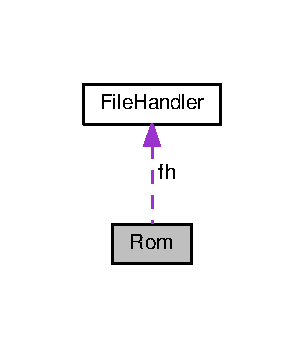
\includegraphics[width=146pt]{classRom__coll__graph}
\end{center}
\end{figure}
\subsection*{Public Member Functions}
\begin{DoxyCompactItemize}
\item 
\hyperlink{classRom_a7ae10e2c40489fc7e5727694dab3e906}{$\sim$\+Rom} ()
\end{DoxyCompactItemize}
\subsection*{Private Member Functions}
\begin{DoxyCompactItemize}
\item 
virtual void \hyperlink{classRom_a427f623e435adbff5e49bfc42018ee17}{b\+\_\+transport} (tlm\+::tlm\+\_\+generic\+\_\+payload \&transaction, sc\+\_\+time \&delay)
\end{DoxyCompactItemize}
\subsection*{Private Attributes}
\begin{DoxyCompactItemize}
\item 
sc\+\_\+int$<$ \hyperlink{Defines_8h_af087b76f9707be9d3b43ba0c782c31c3}{D\+A\+T\+A\+\_\+\+W\+I\+D\+T\+H} $>$ \hyperlink{classRom_aed8f55c20e5ba447c9d312b6bac82dcd}{mem} \mbox{[}\hyperlink{Defines_8h_a3744909059435c19ead1ff15e0fb3257}{R\+O\+M\+\_\+\+D\+E\+P\+T\+H}\mbox{]}
\item 
\hyperlink{classFileHandler}{File\+Handler} $\ast$ \hyperlink{classRom_ad7d70385f6cd68a97c89c48f4590cbb1}{fh}
\end{DoxyCompactItemize}


\subsection{Detailed Description}
Read-\/\+Only Memory. 

Módulo responsável por manter e fazer a interface entre a memória R\+O\+M com os demais módulos.

\begin{DoxyAuthor}{Author}
Gerson Miguel Beckenkamp 
\end{DoxyAuthor}
\begin{DoxyDate}{Date}
2015/09/05 14\+:16\+:20 
\end{DoxyDate}


Definition at line 33 of file Rom.\+h.



\subsection{Constructor \& Destructor Documentation}
\hypertarget{classRom_a7ae10e2c40489fc7e5727694dab3e906}{\index{Rom@{Rom}!````~Rom@{$\sim$\+Rom}}
\index{````~Rom@{$\sim$\+Rom}!Rom@{Rom}}
\subsubsection[{$\sim$\+Rom}]{\setlength{\rightskip}{0pt plus 5cm}Rom\+::$\sim$\+Rom (
\begin{DoxyParamCaption}
{}
\end{DoxyParamCaption}
)}}\label{classRom_a7ae10e2c40489fc7e5727694dab3e906}
Destrutor do módulo. 

Definition at line 68 of file Rom.\+cpp.



\subsection{Member Function Documentation}
\hypertarget{classRom_a427f623e435adbff5e49bfc42018ee17}{\index{Rom@{Rom}!b\+\_\+transport@{b\+\_\+transport}}
\index{b\+\_\+transport@{b\+\_\+transport}!Rom@{Rom}}
\subsubsection[{b\+\_\+transport}]{\setlength{\rightskip}{0pt plus 5cm}void Rom\+::b\+\_\+transport (
\begin{DoxyParamCaption}
\item[{tlm\+::tlm\+\_\+generic\+\_\+payload \&}]{trans, }
\item[{sc\+\_\+time \&}]{delay}
\end{DoxyParamCaption}
)\hspace{0.3cm}{\ttfamily [private]}, {\ttfamily [virtual]}}}\label{classRom_a427f623e435adbff5e49bfc42018ee17}
Socket responsável por receber requerimentos de leitura do módulo \hyperlink{classFetch}{Fetch}. 
\begin{DoxyParams}{Parameters}
{\em trans} & Payload contendo os dados do pacote recebido. \\
\hline
{\em delay} & Timeout para a condirmação do comando recebido. \\
\hline
\end{DoxyParams}
\begin{DoxyReturn}{Returns}
Não há retorno. 
\end{DoxyReturn}


Definition at line 28 of file Rom.\+cpp.



References mem, and S\+I\+Z\+E.



\subsection{Member Data Documentation}
\hypertarget{classRom_ad7d70385f6cd68a97c89c48f4590cbb1}{\index{Rom@{Rom}!fh@{fh}}
\index{fh@{fh}!Rom@{Rom}}
\subsubsection[{fh}]{\setlength{\rightskip}{0pt plus 5cm}{\bf File\+Handler}$\ast$ Rom\+::fh\hspace{0.3cm}{\ttfamily [private]}}}\label{classRom_ad7d70385f6cd68a97c89c48f4590cbb1}
Gerenciador de arquivos. 

Definition at line 37 of file Rom.\+h.

\hypertarget{classRom_aed8f55c20e5ba447c9d312b6bac82dcd}{\index{Rom@{Rom}!mem@{mem}}
\index{mem@{mem}!Rom@{Rom}}
\subsubsection[{mem}]{\setlength{\rightskip}{0pt plus 5cm}sc\+\_\+int$<${\bf D\+A\+T\+A\+\_\+\+W\+I\+D\+T\+H}$>$ Rom\+::mem\mbox{[}{\bf R\+O\+M\+\_\+\+D\+E\+P\+T\+H}\mbox{]}\hspace{0.3cm}{\ttfamily [private]}}}\label{classRom_aed8f55c20e5ba447c9d312b6bac82dcd}
Memória R\+O\+M. 

Definition at line 36 of file Rom.\+h.



Referenced by b\+\_\+transport().



The documentation for this class was generated from the following files\+:\begin{DoxyCompactItemize}
\item 
\hyperlink{Rom_8h}{Rom.\+h}\item 
\hyperlink{Rom_8cpp}{Rom.\+cpp}\end{DoxyCompactItemize}

\hypertarget{classStack}{\section{Stack Class Reference}
\label{classStack}\index{Stack@{Stack}}
}


Pilha de retorno.  




{\ttfamily \#include $<$Return\+Stack.\+h$>$}



Inherits sc\+\_\+module.

\subsection*{Public Member Functions}
\begin{DoxyCompactItemize}
\item 
void \hyperlink{classStack_a9307cd8107283c08c080b22bdd66d196}{set\+Buffers} (int $\ast$buf)
\item 
\hyperlink{classStack_a40bd5dff912f0e5290777c4b46d17809}{$\sim$\+Stack} ()
\end{DoxyCompactItemize}
\subsection*{Private Member Functions}
\begin{DoxyCompactItemize}
\item 
virtual void \hyperlink{classStack_a188c0ef6d86bb6100b6c1a63e821bd7f}{b\+\_\+transport} (tlm\+::tlm\+\_\+generic\+\_\+payload \&trans, sc\+\_\+time \&delay)
\item 
void \hyperlink{classStack_a5c98f94f6a3a5384c754794b1aebb724}{update\+Buffers} ()
\end{DoxyCompactItemize}


\subsection{Detailed Description}
Pilha de retorno. 

Módulo responsável por manter e fazer a interface da pilha de retorno com os demais blocos.

\begin{DoxyAuthor}{Author}
Gerson Miguel Beckenkamp 
\end{DoxyAuthor}
\begin{DoxyDate}{Date}
2015/09/05 14\+:16\+:20 
\end{DoxyDate}


Definition at line 33 of file Return\+Stack.\+h.



\subsection{Constructor \& Destructor Documentation}
\hypertarget{classStack_a40bd5dff912f0e5290777c4b46d17809}{\index{Stack@{Stack}!````~Stack@{$\sim$\+Stack}}
\index{````~Stack@{$\sim$\+Stack}!Stack@{Stack}}
\subsubsection[{$\sim$\+Stack}]{\setlength{\rightskip}{0pt plus 5cm}Stack\+::$\sim$\+Stack (
\begin{DoxyParamCaption}
{}
\end{DoxyParamCaption}
)}}\label{classStack_a40bd5dff912f0e5290777c4b46d17809}
Destrudor do módulo. 

Definition at line 131 of file Return\+Stack.\+cpp.



\subsection{Member Function Documentation}
\hypertarget{classStack_a188c0ef6d86bb6100b6c1a63e821bd7f}{\index{Stack@{Stack}!b\+\_\+transport@{b\+\_\+transport}}
\index{b\+\_\+transport@{b\+\_\+transport}!Stack@{Stack}}
\subsubsection[{b\+\_\+transport}]{\setlength{\rightskip}{0pt plus 5cm}void Stack\+::b\+\_\+transport (
\begin{DoxyParamCaption}
\item[{tlm\+::tlm\+\_\+generic\+\_\+payload \&}]{trans, }
\item[{sc\+\_\+time \&}]{delay}
\end{DoxyParamCaption}
)\hspace{0.3cm}{\ttfamily [private]}, {\ttfamily [virtual]}}}\label{classStack_a188c0ef6d86bb6100b6c1a63e821bd7f}
Socket responsável por receber requisições oriundas da \hyperlink{classAlu}{Alu}. 
\begin{DoxyParams}{Parameters}
{\em trans} & Payload contendo os dados do pacote recebido. \\
\hline
{\em delay} & Timeout para a condirmação do comando recebido. \\
\hline
\end{DoxyParams}
\begin{DoxyReturn}{Returns}
Não há retorno. 
\end{DoxyReturn}


Definition at line 26 of file Return\+Stack.\+cpp.



References D\+S\+\_\+\+S\+I\+Z\+E, S\+I\+Z\+E, and update\+Buffers().

\hypertarget{classStack_a9307cd8107283c08c080b22bdd66d196}{\index{Stack@{Stack}!set\+Buffers@{set\+Buffers}}
\index{set\+Buffers@{set\+Buffers}!Stack@{Stack}}
\subsubsection[{set\+Buffers}]{\setlength{\rightskip}{0pt plus 5cm}void Stack\+::set\+Buffers (
\begin{DoxyParamCaption}
\item[{int $\ast$}]{buf}
\end{DoxyParamCaption}
)}}\label{classStack_a9307cd8107283c08c080b22bdd66d196}
Inicia os buffers de topo de pilha.

\begin{DoxyReturn}{Returns}
Não há retorno. 
\end{DoxyReturn}


Definition at line 124 of file Return\+Stack.\+cpp.



Referenced by S\+C\+\_\+\+M\+O\+D\+U\+L\+E().

\hypertarget{classStack_a5c98f94f6a3a5384c754794b1aebb724}{\index{Stack@{Stack}!update\+Buffers@{update\+Buffers}}
\index{update\+Buffers@{update\+Buffers}!Stack@{Stack}}
\subsubsection[{update\+Buffers}]{\setlength{\rightskip}{0pt plus 5cm}void Stack\+::update\+Buffers (
\begin{DoxyParamCaption}
{}
\end{DoxyParamCaption}
)\hspace{0.3cm}{\ttfamily [private]}}}\label{classStack_a5c98f94f6a3a5384c754794b1aebb724}
Executa a sincronização dos buffers com o topo da pilha.

\begin{DoxyReturn}{Returns}
Não há retorno. 
\end{DoxyReturn}


Definition at line 109 of file Return\+Stack.\+cpp.



Referenced by b\+\_\+transport().



The documentation for this class was generated from the following files\+:\begin{DoxyCompactItemize}
\item 
\hyperlink{ReturnStack_8h}{Return\+Stack.\+h}\item 
\hyperlink{ReturnStack_8cpp}{Return\+Stack.\+cpp}\end{DoxyCompactItemize}

\chapter{File Documentation}
\hypertarget{Alu_8cpp}{\section{Alu.\+cpp File Reference}
\label{Alu_8cpp}\index{Alu.\+cpp@{Alu.\+cpp}}
}
{\ttfamily \#include \char`\"{}Alu.\+h\char`\"{}}\\*
Include dependency graph for Alu.\+cpp\+:\nopagebreak
\begin{figure}[H]
\begin{center}
\leavevmode
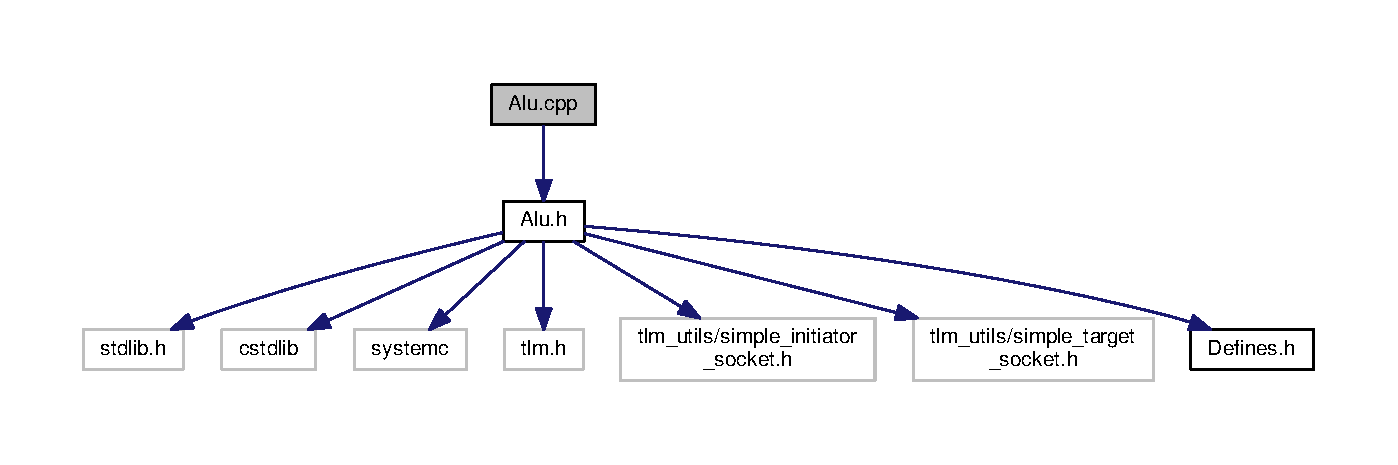
\includegraphics[width=350pt]{Alu_8cpp__incl}
\end{center}
\end{figure}

\hypertarget{Alu_8h}{\section{Alu.\+h File Reference}
\label{Alu_8h}\index{Alu.\+h@{Alu.\+h}}
}
{\ttfamily \#include $<$stdlib.\+h$>$}\\*
{\ttfamily \#include $<$cstdlib$>$}\\*
{\ttfamily \#include \char`\"{}systemc\char`\"{}}\\*
{\ttfamily \#include \char`\"{}tlm.\+h\char`\"{}}\\*
{\ttfamily \#include \char`\"{}tlm\+\_\+utils/simple\+\_\+initiator\+\_\+socket.\+h\char`\"{}}\\*
{\ttfamily \#include \char`\"{}tlm\+\_\+utils/simple\+\_\+target\+\_\+socket.\+h\char`\"{}}\\*
{\ttfamily \#include \char`\"{}Defines.\+h\char`\"{}}\\*
Include dependency graph for Alu.\+h\+:\nopagebreak
\begin{figure}[H]
\begin{center}
\leavevmode
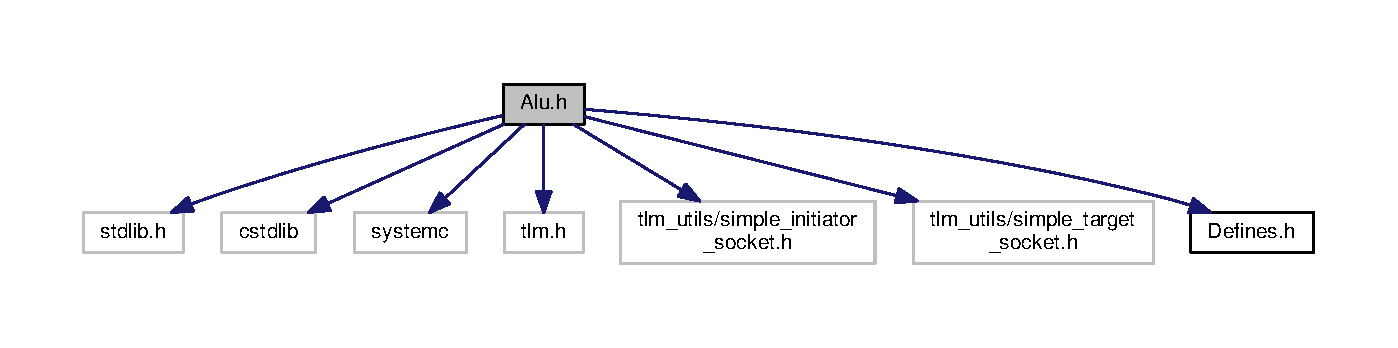
\includegraphics[width=350pt]{Alu_8h__incl}
\end{center}
\end{figure}
This graph shows which files directly or indirectly include this file\+:\nopagebreak
\begin{figure}[H]
\begin{center}
\leavevmode
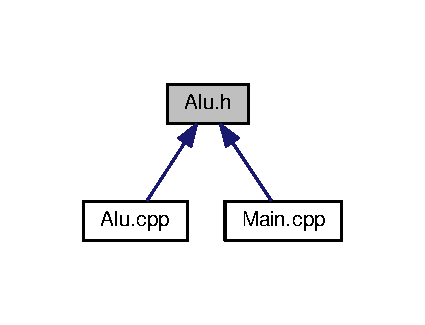
\includegraphics[width=204pt]{Alu_8h__dep__incl}
\end{center}
\end{figure}
\subsection*{Classes}
\begin{DoxyCompactItemize}
\item 
class \hyperlink{classAlu}{Alu}
\begin{DoxyCompactList}\small\item\em Unidade Lógico Aritmética. \end{DoxyCompactList}\end{DoxyCompactItemize}

\hypertarget{DataStack_8cpp}{\section{Data\+Stack.\+cpp File Reference}
\label{DataStack_8cpp}\index{Data\+Stack.\+cpp@{Data\+Stack.\+cpp}}
}
{\ttfamily \#include \char`\"{}Data\+Stack.\+h\char`\"{}}\\*
Include dependency graph for Data\+Stack.\+cpp\+:\nopagebreak
\begin{figure}[H]
\begin{center}
\leavevmode
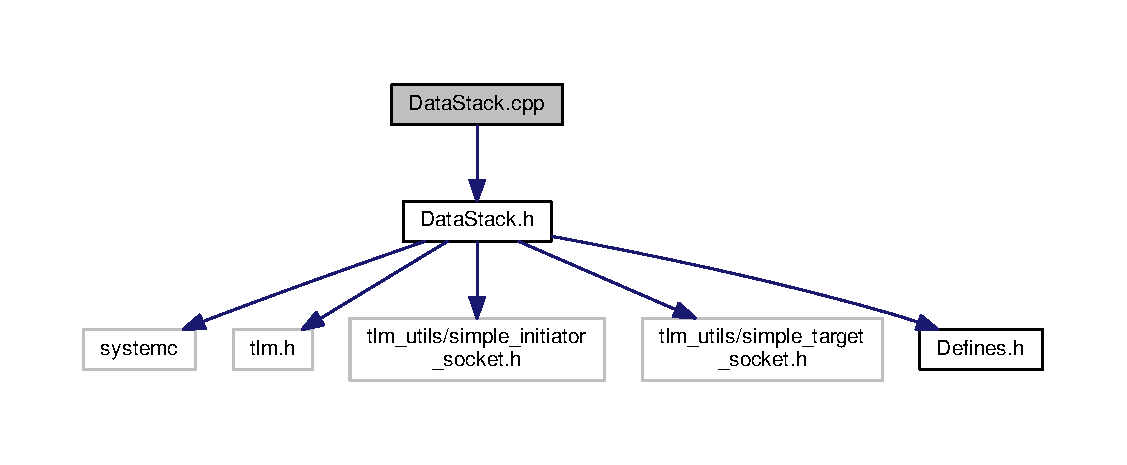
\includegraphics[width=350pt]{DataStack_8cpp__incl}
\end{center}
\end{figure}

\hypertarget{DataStack_8h}{\section{Data\+Stack.\+h File Reference}
\label{DataStack_8h}\index{Data\+Stack.\+h@{Data\+Stack.\+h}}
}
{\ttfamily \#include \char`\"{}systemc\char`\"{}}\\*
{\ttfamily \#include \char`\"{}tlm.\+h\char`\"{}}\\*
{\ttfamily \#include \char`\"{}tlm\+\_\+utils/simple\+\_\+initiator\+\_\+socket.\+h\char`\"{}}\\*
{\ttfamily \#include \char`\"{}tlm\+\_\+utils/simple\+\_\+target\+\_\+socket.\+h\char`\"{}}\\*
{\ttfamily \#include \char`\"{}Defines.\+h\char`\"{}}\\*
Include dependency graph for Data\+Stack.\+h\+:\nopagebreak
\begin{figure}[H]
\begin{center}
\leavevmode
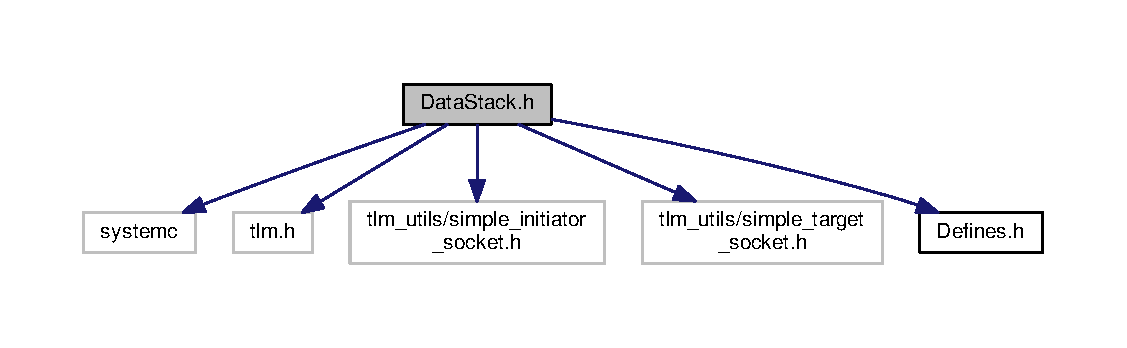
\includegraphics[width=350pt]{DataStack_8h__incl}
\end{center}
\end{figure}
This graph shows which files directly or indirectly include this file\+:\nopagebreak
\begin{figure}[H]
\begin{center}
\leavevmode
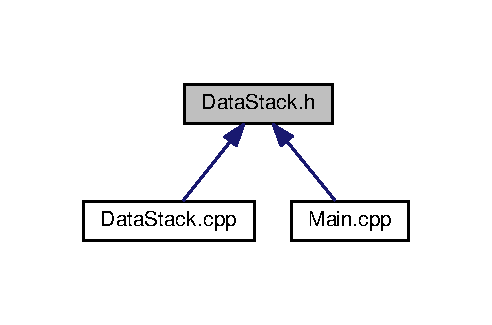
\includegraphics[width=236pt]{DataStack_8h__dep__incl}
\end{center}
\end{figure}
\subsection*{Classes}
\begin{DoxyCompactItemize}
\item 
class \hyperlink{classDataStack}{Data\+Stack}
\begin{DoxyCompactList}\small\item\em Pilha de dados. \end{DoxyCompactList}\end{DoxyCompactItemize}

\hypertarget{Defines_8h}{\section{Defines.\+h File Reference}
\label{Defines_8h}\index{Defines.\+h@{Defines.\+h}}
}


Definição de valores fixos do sistema.  


This graph shows which files directly or indirectly include this file\+:\nopagebreak
\begin{figure}[H]
\begin{center}
\leavevmode
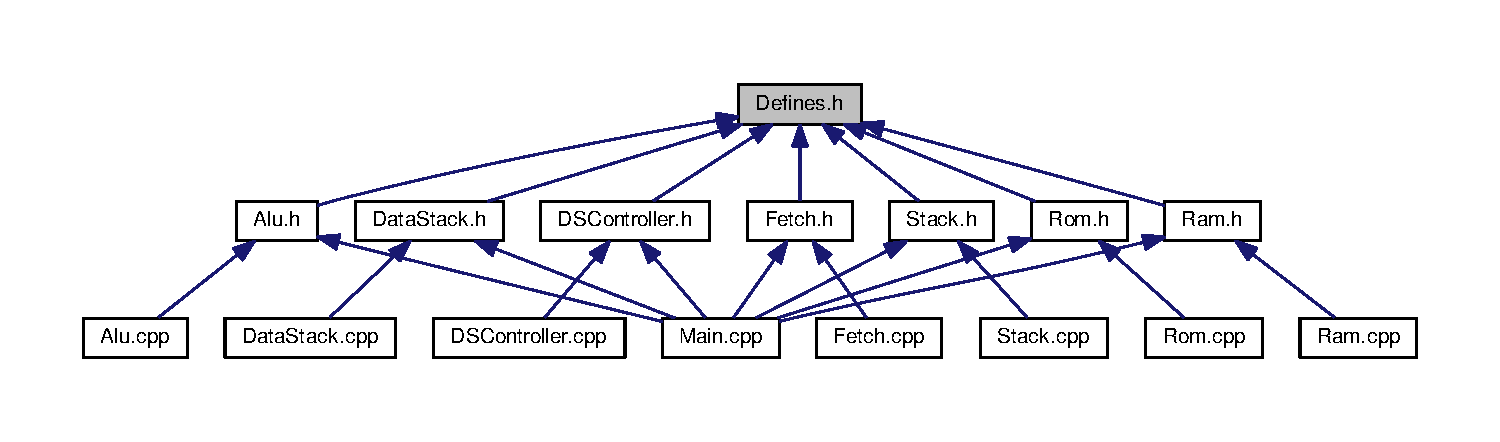
\includegraphics[width=350pt]{Defines_8h__dep__incl}
\end{center}
\end{figure}
\subsection*{Macros}
\begin{DoxyCompactItemize}
\item 
\hypertarget{Defines_8h_ab0139008fdda107456f13f837872b410}{\#define \hyperlink{Defines_8h_ab0139008fdda107456f13f837872b410}{P\+A\+T\+H}~\char`\"{}program.\+sm\char`\"{}}\label{Defines_8h_ab0139008fdda107456f13f837872b410}

\begin{DoxyCompactList}\small\item\em Caminho para o arquivo de programa. \end{DoxyCompactList}\item 
\hypertarget{Defines_8h_ac8566d115f5d53e0c4f4cf7b2eab21b9}{\#define \hyperlink{Defines_8h_ac8566d115f5d53e0c4f4cf7b2eab21b9}{D\+E\+B\+U\+G\+\_\+\+P\+R\+I\+N\+T\+\_\+\+R\+A\+M\+\_\+\+T\+O\+P}~32}\label{Defines_8h_ac8566d115f5d53e0c4f4cf7b2eab21b9}

\begin{DoxyCompactList}\small\item\em Topo do bloco de R\+A\+M que será exibido. \end{DoxyCompactList}\item 
\hypertarget{Defines_8h_a152535ea72994340af931bdfe1c15fbd}{\#define \hyperlink{Defines_8h_a152535ea72994340af931bdfe1c15fbd}{D\+E\+B\+U\+G\+\_\+\+P\+R\+I\+N\+T\+\_\+\+R\+A\+M\+\_\+\+D\+O\+W\+N}~0}\label{Defines_8h_a152535ea72994340af931bdfe1c15fbd}

\begin{DoxyCompactList}\small\item\em Base do bloco de R\+A\+M que será exibido. \end{DoxyCompactList}\item 
\hypertarget{Defines_8h_a70ed59adcb4159ac551058053e649640}{\#define \hyperlink{Defines_8h_a70ed59adcb4159ac551058053e649640}{S\+I\+Z\+E}~256}\label{Defines_8h_a70ed59adcb4159ac551058053e649640}

\begin{DoxyCompactList}\small\item\em Data size. \end{DoxyCompactList}\item 
\hypertarget{Defines_8h_af087b76f9707be9d3b43ba0c782c31c3}{\#define \hyperlink{Defines_8h_af087b76f9707be9d3b43ba0c782c31c3}{D\+A\+T\+A\+\_\+\+W\+I\+D\+T\+H}~32}\label{Defines_8h_af087b76f9707be9d3b43ba0c782c31c3}

\begin{DoxyCompactList}\small\item\em Tamanho da palavra do sistema. \end{DoxyCompactList}\item 
\hypertarget{Defines_8h_ab683dabe89fc48ada1209e0e3733862a}{\#define \hyperlink{Defines_8h_ab683dabe89fc48ada1209e0e3733862a}{R\+A\+M\+\_\+\+D\+E\+P\+T\+H}~128}\label{Defines_8h_ab683dabe89fc48ada1209e0e3733862a}

\begin{DoxyCompactList}\small\item\em Tamanho da memória R\+A\+M. \end{DoxyCompactList}\item 
\hypertarget{Defines_8h_a3744909059435c19ead1ff15e0fb3257}{\#define \hyperlink{Defines_8h_a3744909059435c19ead1ff15e0fb3257}{R\+O\+M\+\_\+\+D\+E\+P\+T\+H}~128}\label{Defines_8h_a3744909059435c19ead1ff15e0fb3257}

\begin{DoxyCompactList}\small\item\em Tamanho da memória R\+O\+M. \end{DoxyCompactList}\item 
\hypertarget{Defines_8h_a6423a880df59733d2d9b509c7718d3a9}{\#define \hyperlink{Defines_8h_a6423a880df59733d2d9b509c7718d3a9}{S\+T\+A\+C\+K\+\_\+\+S\+I\+Z\+E}~16}\label{Defines_8h_a6423a880df59733d2d9b509c7718d3a9}

\begin{DoxyCompactList}\small\item\em Tamanho máximo de pilha suportado. \end{DoxyCompactList}\item 
\hypertarget{Defines_8h_ad5e508a5b19bccfd53ac0ec31800a512}{\#define \hyperlink{Defines_8h_ad5e508a5b19bccfd53ac0ec31800a512}{D\+S\+\_\+\+S\+I\+Z\+E}~8}\label{Defines_8h_ad5e508a5b19bccfd53ac0ec31800a512}

\begin{DoxyCompactList}\small\item\em Tamanho atual da pilha de dados. \end{DoxyCompactList}\item 
\hypertarget{Defines_8h_aaa916e8a6bf8f5df13e12be1c6eefead}{\#define \hyperlink{Defines_8h_aaa916e8a6bf8f5df13e12be1c6eefead}{R\+S\+\_\+\+S\+I\+Z\+E}~8}\label{Defines_8h_aaa916e8a6bf8f5df13e12be1c6eefead}

\begin{DoxyCompactList}\small\item\em Tamanho atual da pilha de retorno. \end{DoxyCompactList}\end{DoxyCompactItemize}


\subsection{Detailed Description}
Definição de valores fixos do sistema. 

\begin{DoxyAuthor}{Author}
Gerson Miguel Beckenkamp 
\end{DoxyAuthor}
\begin{DoxyDate}{Date}
2015/09/05 14\+:16\+:20 
\end{DoxyDate}


Definition in file \hyperlink{Defines_8h_source}{Defines.\+h}.


\hypertarget{DSController_8cpp}{\section{D\+S\+Controller.\+cpp File Reference}
\label{DSController_8cpp}\index{D\+S\+Controller.\+cpp@{D\+S\+Controller.\+cpp}}
}
{\ttfamily \#include \char`\"{}D\+S\+Controller.\+h\char`\"{}}\\*
Include dependency graph for D\+S\+Controller.\+cpp\+:\nopagebreak
\begin{figure}[H]
\begin{center}
\leavevmode
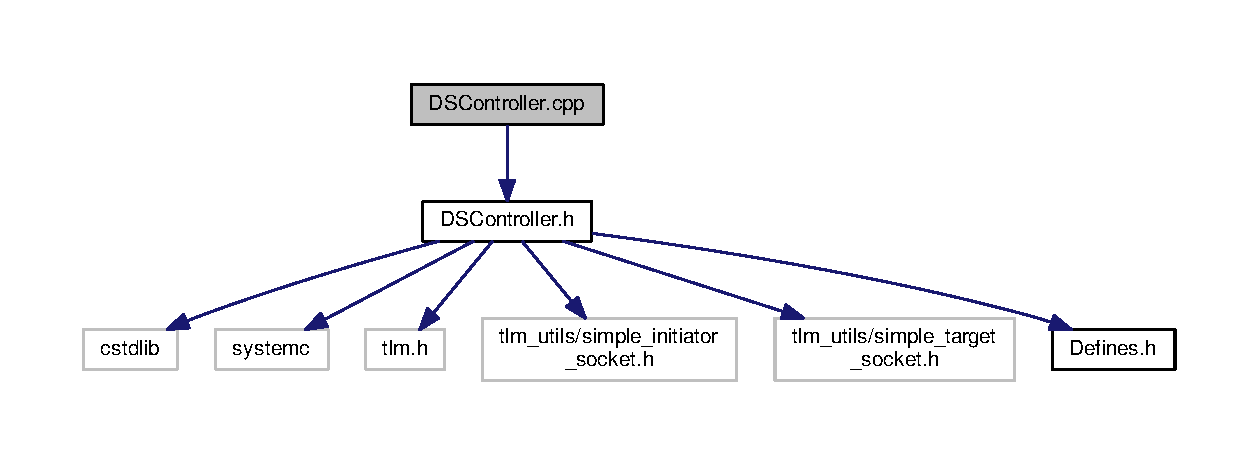
\includegraphics[width=350pt]{DSController_8cpp__incl}
\end{center}
\end{figure}

\hypertarget{DSController_8h}{\section{D\+S\+Controller.\+h File Reference}
\label{DSController_8h}\index{D\+S\+Controller.\+h@{D\+S\+Controller.\+h}}
}
{\ttfamily \#include $<$cstdlib$>$}\\*
{\ttfamily \#include \char`\"{}systemc\char`\"{}}\\*
{\ttfamily \#include \char`\"{}tlm.\+h\char`\"{}}\\*
{\ttfamily \#include \char`\"{}tlm\+\_\+utils/simple\+\_\+initiator\+\_\+socket.\+h\char`\"{}}\\*
{\ttfamily \#include \char`\"{}tlm\+\_\+utils/simple\+\_\+target\+\_\+socket.\+h\char`\"{}}\\*
{\ttfamily \#include \char`\"{}Defines.\+h\char`\"{}}\\*
Include dependency graph for D\+S\+Controller.\+h\+:\nopagebreak
\begin{figure}[H]
\begin{center}
\leavevmode
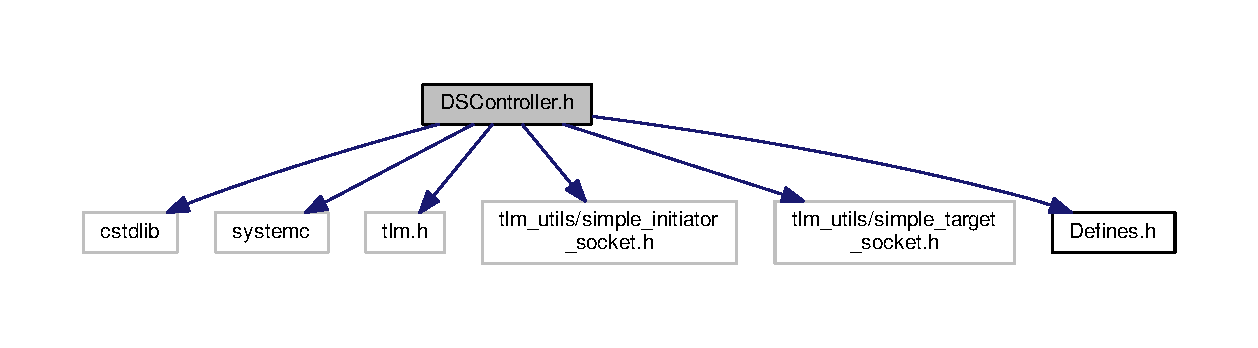
\includegraphics[width=350pt]{DSController_8h__incl}
\end{center}
\end{figure}
This graph shows which files directly or indirectly include this file\+:\nopagebreak
\begin{figure}[H]
\begin{center}
\leavevmode
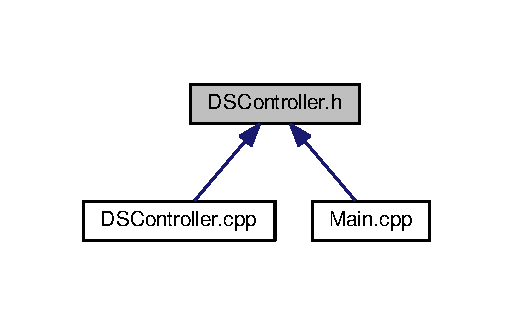
\includegraphics[width=246pt]{DSController_8h__dep__incl}
\end{center}
\end{figure}
\subsection*{Classes}
\begin{DoxyCompactItemize}
\item 
class \hyperlink{classDSController}{D\+S\+Controller}
\begin{DoxyCompactList}\small\item\em Controlador da pilha de dados. \end{DoxyCompactList}\end{DoxyCompactItemize}

\hypertarget{Fetch_8cpp}{\section{Fetch.\+cpp File Reference}
\label{Fetch_8cpp}\index{Fetch.\+cpp@{Fetch.\+cpp}}
}
{\ttfamily \#include \char`\"{}Fetch.\+h\char`\"{}}\\*
Include dependency graph for Fetch.\+cpp\+:\nopagebreak
\begin{figure}[H]
\begin{center}
\leavevmode
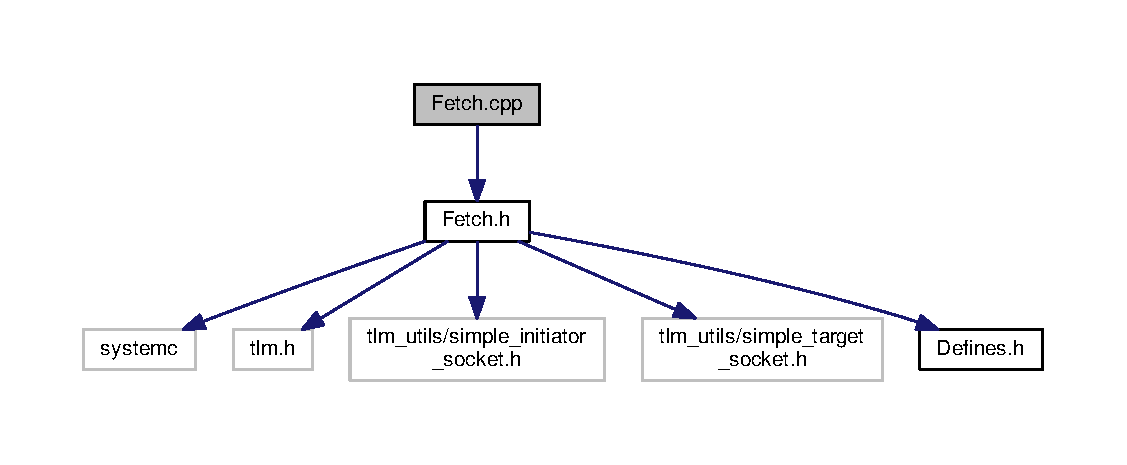
\includegraphics[width=350pt]{Fetch_8cpp__incl}
\end{center}
\end{figure}

\hypertarget{Fetch_8h}{\section{Fetch.\+h File Reference}
\label{Fetch_8h}\index{Fetch.\+h@{Fetch.\+h}}
}
{\ttfamily \#include \char`\"{}systemc\char`\"{}}\\*
{\ttfamily \#include \char`\"{}tlm.\+h\char`\"{}}\\*
{\ttfamily \#include \char`\"{}tlm\+\_\+utils/simple\+\_\+initiator\+\_\+socket.\+h\char`\"{}}\\*
{\ttfamily \#include \char`\"{}tlm\+\_\+utils/simple\+\_\+target\+\_\+socket.\+h\char`\"{}}\\*
{\ttfamily \#include \char`\"{}Defines.\+h\char`\"{}}\\*
Include dependency graph for Fetch.\+h\+:\nopagebreak
\begin{figure}[H]
\begin{center}
\leavevmode
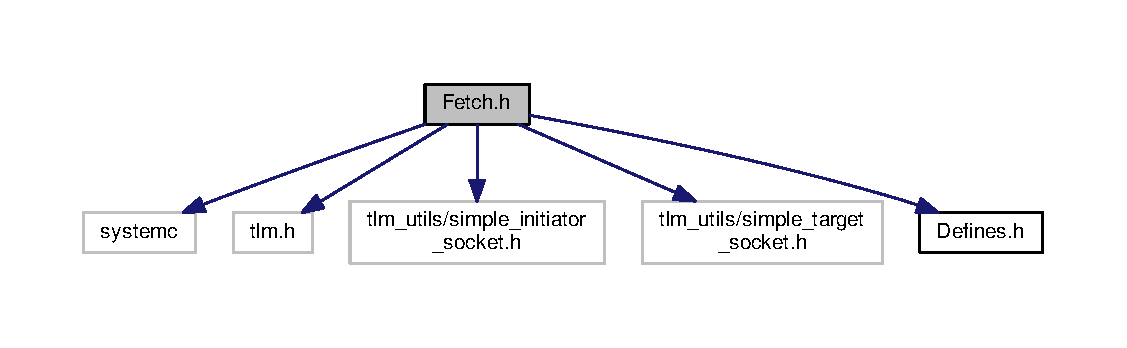
\includegraphics[width=350pt]{Fetch_8h__incl}
\end{center}
\end{figure}
This graph shows which files directly or indirectly include this file\+:\nopagebreak
\begin{figure}[H]
\begin{center}
\leavevmode
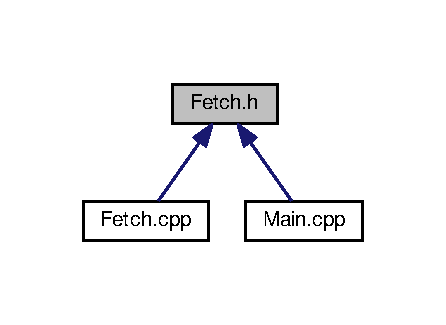
\includegraphics[width=214pt]{Fetch_8h__dep__incl}
\end{center}
\end{figure}
\subsection*{Classes}
\begin{DoxyCompactItemize}
\item 
class \hyperlink{classFetch}{Fetch}
\begin{DoxyCompactList}\small\item\em Interface da R\+O\+M com o resto do sistema. \end{DoxyCompactList}\end{DoxyCompactItemize}

\hypertarget{FileHandler_8cpp}{\section{File\+Handler.\+cpp File Reference}
\label{FileHandler_8cpp}\index{File\+Handler.\+cpp@{File\+Handler.\+cpp}}
}
{\ttfamily \#include \char`\"{}systemc\char`\"{}}\\*
{\ttfamily \#include $<$iostream$>$}\\*
{\ttfamily \#include $<$sstream$>$}\\*
{\ttfamily \#include $<$fstream$>$}\\*
{\ttfamily \#include $<$string$>$}\\*
{\ttfamily \#include $<$bitset$>$}\\*
Include dependency graph for File\+Handler.\+cpp\+:\nopagebreak
\begin{figure}[H]
\begin{center}
\leavevmode
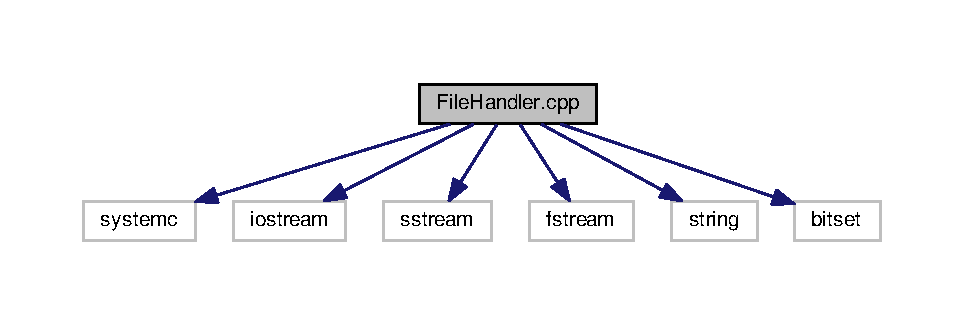
\includegraphics[width=350pt]{FileHandler_8cpp__incl}
\end{center}
\end{figure}
This graph shows which files directly or indirectly include this file\+:\nopagebreak
\begin{figure}[H]
\begin{center}
\leavevmode
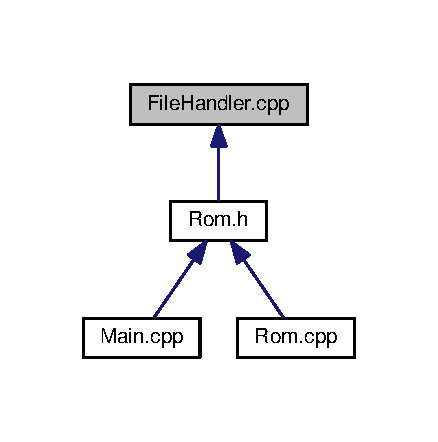
\includegraphics[width=210pt]{FileHandler_8cpp__dep__incl}
\end{center}
\end{figure}
\subsection*{Classes}
\begin{DoxyCompactItemize}
\item 
class \hyperlink{classFileHandler}{File\+Handler}
\begin{DoxyCompactList}\small\item\em Gerenciador de arquivos. \end{DoxyCompactList}\end{DoxyCompactItemize}

\hypertarget{Main_8cpp}{\section{Main.\+cpp File Reference}
\label{Main_8cpp}\index{Main.\+cpp@{Main.\+cpp}}
}


Método main.  


{\ttfamily \#include \char`\"{}systemc\char`\"{}}\\*
{\ttfamily \#include $<$iostream$>$}\\*
{\ttfamily \#include \char`\"{}Stack.\+h\char`\"{}}\\*
{\ttfamily \#include \char`\"{}Data\+Stack.\+h\char`\"{}}\\*
{\ttfamily \#include \char`\"{}Rom.\+h\char`\"{}}\\*
{\ttfamily \#include \char`\"{}D\+S\+Controller.\+h\char`\"{}}\\*
{\ttfamily \#include \char`\"{}Fetch.\+h\char`\"{}}\\*
{\ttfamily \#include \char`\"{}Alu.\+h\char`\"{}}\\*
{\ttfamily \#include \char`\"{}Ram.\+h\char`\"{}}\\*
{\ttfamily \#include \char`\"{}tlm.\+h\char`\"{}}\\*
{\ttfamily \#include \char`\"{}tlm\+\_\+utils/simple\+\_\+initiator\+\_\+socket.\+h\char`\"{}}\\*
{\ttfamily \#include \char`\"{}tlm\+\_\+utils/simple\+\_\+target\+\_\+socket.\+h\char`\"{}}\\*
Include dependency graph for Main.\+cpp\+:\nopagebreak
\begin{figure}[H]
\begin{center}
\leavevmode
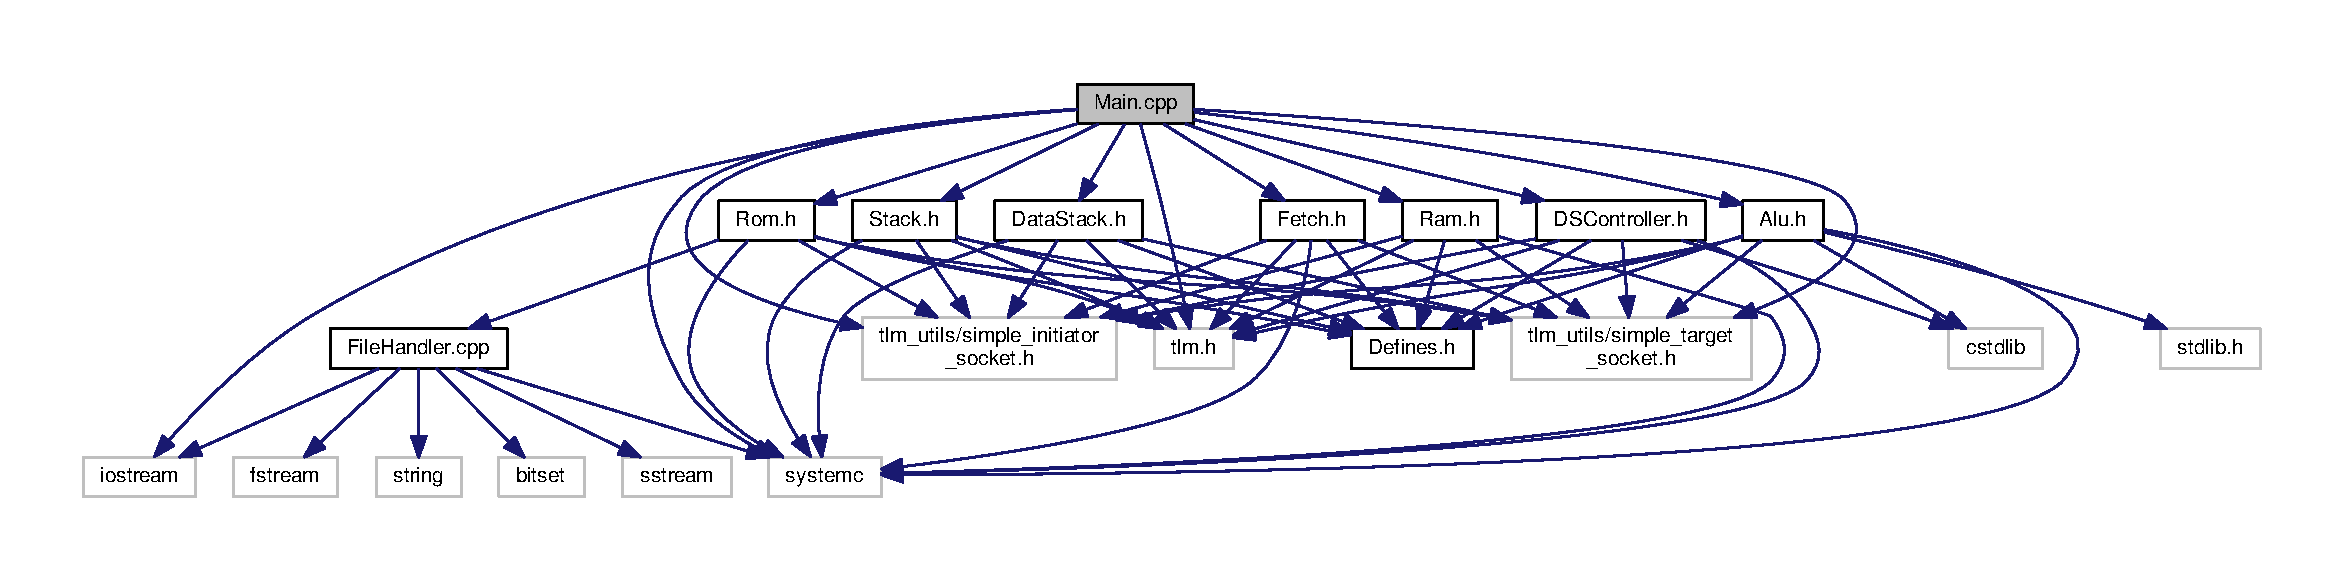
\includegraphics[width=350pt]{Main_8cpp__incl}
\end{center}
\end{figure}
\subsection*{Functions}
\begin{DoxyCompactItemize}
\item 
\hyperlink{Main_8cpp_aa33fdde3e142343f881ee209c8faa135}{S\+C\+\_\+\+M\+O\+D\+U\+L\+E} (Top)
\end{DoxyCompactItemize}


\subsection{Detailed Description}
Método main. 

\begin{DoxyAuthor}{Author}
Gerson Miguel Beckenkamp 
\end{DoxyAuthor}
\begin{DoxyDate}{Date}
2015/09/05 14\+:16\+:20 
\end{DoxyDate}


Definition in file \hyperlink{Main_8cpp_source}{Main.\+cpp}.



\subsection{Function Documentation}
\hypertarget{Main_8cpp_aa33fdde3e142343f881ee209c8faa135}{\index{Main.\+cpp@{Main.\+cpp}!S\+C\+\_\+\+M\+O\+D\+U\+L\+E@{S\+C\+\_\+\+M\+O\+D\+U\+L\+E}}
\index{S\+C\+\_\+\+M\+O\+D\+U\+L\+E@{S\+C\+\_\+\+M\+O\+D\+U\+L\+E}!Main.\+cpp@{Main.\+cpp}}
\subsubsection[{S\+C\+\_\+\+M\+O\+D\+U\+L\+E}]{\setlength{\rightskip}{0pt plus 5cm}S\+C\+\_\+\+M\+O\+D\+U\+L\+E (
\begin{DoxyParamCaption}
\item[{Top}]{}
\end{DoxyParamCaption}
)}}\label{Main_8cpp_aa33fdde3e142343f881ee209c8faa135}
Módulo de sistema, contendo todos os demais módulos do projeto, bem como suas ligações. 

Definition at line 21 of file Main.\+cpp.



References Ram\+::set\+Cnt(), Fetch\+::set\+Cnt(), Fetch\+::set\+P\+C(), and Alu\+::set\+P\+C().


\hypertarget{Ram_8cpp}{\section{Ram.\+cpp File Reference}
\label{Ram_8cpp}\index{Ram.\+cpp@{Ram.\+cpp}}
}
{\ttfamily \#include \char`\"{}Ram.\+h\char`\"{}}\\*
Include dependency graph for Ram.\+cpp\+:\nopagebreak
\begin{figure}[H]
\begin{center}
\leavevmode
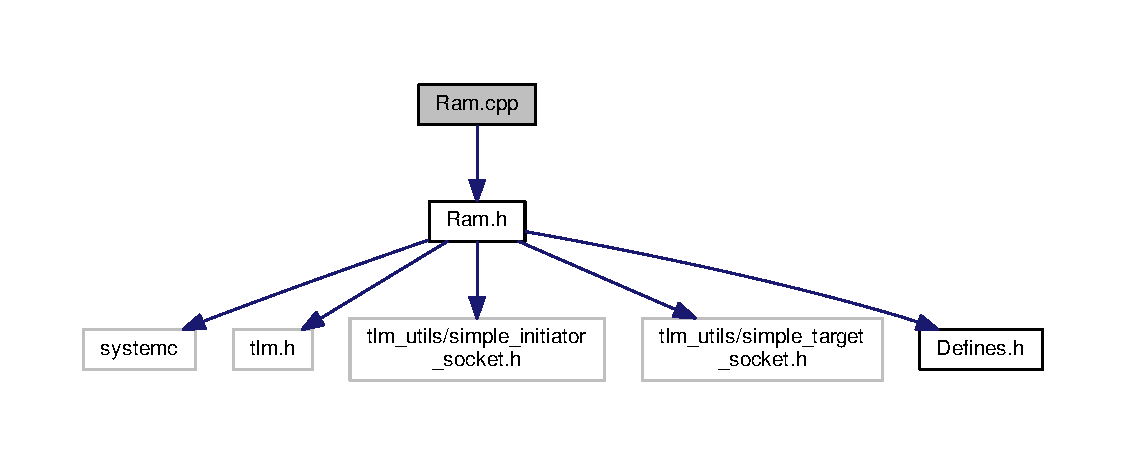
\includegraphics[width=350pt]{Ram_8cpp__incl}
\end{center}
\end{figure}

\hypertarget{Ram_8h}{\section{Ram.\+h File Reference}
\label{Ram_8h}\index{Ram.\+h@{Ram.\+h}}
}
{\ttfamily \#include \char`\"{}systemc\char`\"{}}\\*
{\ttfamily \#include \char`\"{}tlm.\+h\char`\"{}}\\*
{\ttfamily \#include \char`\"{}tlm\+\_\+utils/simple\+\_\+initiator\+\_\+socket.\+h\char`\"{}}\\*
{\ttfamily \#include \char`\"{}tlm\+\_\+utils/simple\+\_\+target\+\_\+socket.\+h\char`\"{}}\\*
{\ttfamily \#include \char`\"{}Defines.\+h\char`\"{}}\\*
Include dependency graph for Ram.\+h\+:\nopagebreak
\begin{figure}[H]
\begin{center}
\leavevmode
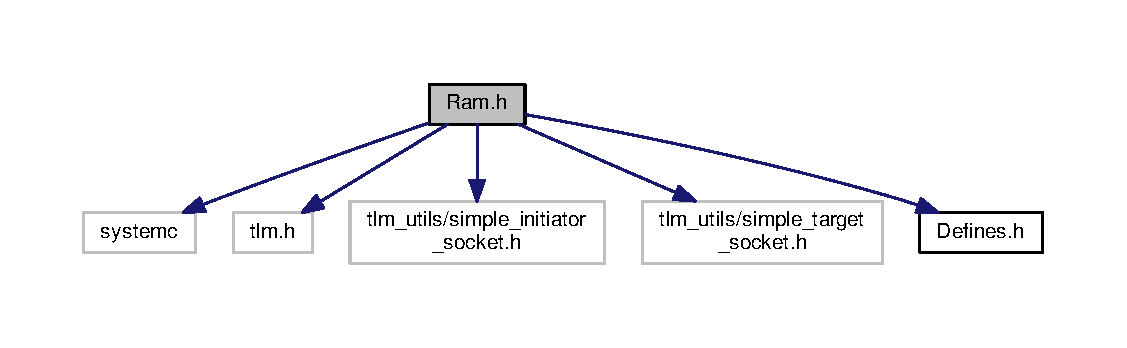
\includegraphics[width=350pt]{Ram_8h__incl}
\end{center}
\end{figure}
This graph shows which files directly or indirectly include this file\+:\nopagebreak
\begin{figure}[H]
\begin{center}
\leavevmode
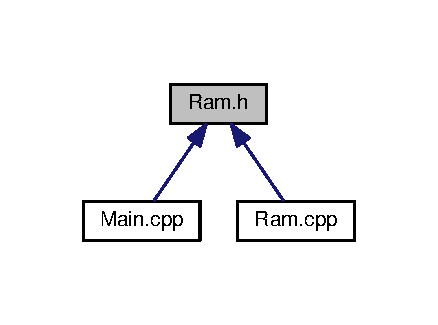
\includegraphics[width=210pt]{Ram_8h__dep__incl}
\end{center}
\end{figure}
\subsection*{Classes}
\begin{DoxyCompactItemize}
\item 
class \hyperlink{classRam}{Ram}
\begin{DoxyCompactList}\small\item\em Random Access Memory. \end{DoxyCompactList}\end{DoxyCompactItemize}

\hypertarget{Rom_8cpp}{\section{Rom.\+cpp File Reference}
\label{Rom_8cpp}\index{Rom.\+cpp@{Rom.\+cpp}}
}
{\ttfamily \#include \char`\"{}Rom.\+h\char`\"{}}\\*
Include dependency graph for Rom.\+cpp\+:\nopagebreak
\begin{figure}[H]
\begin{center}
\leavevmode
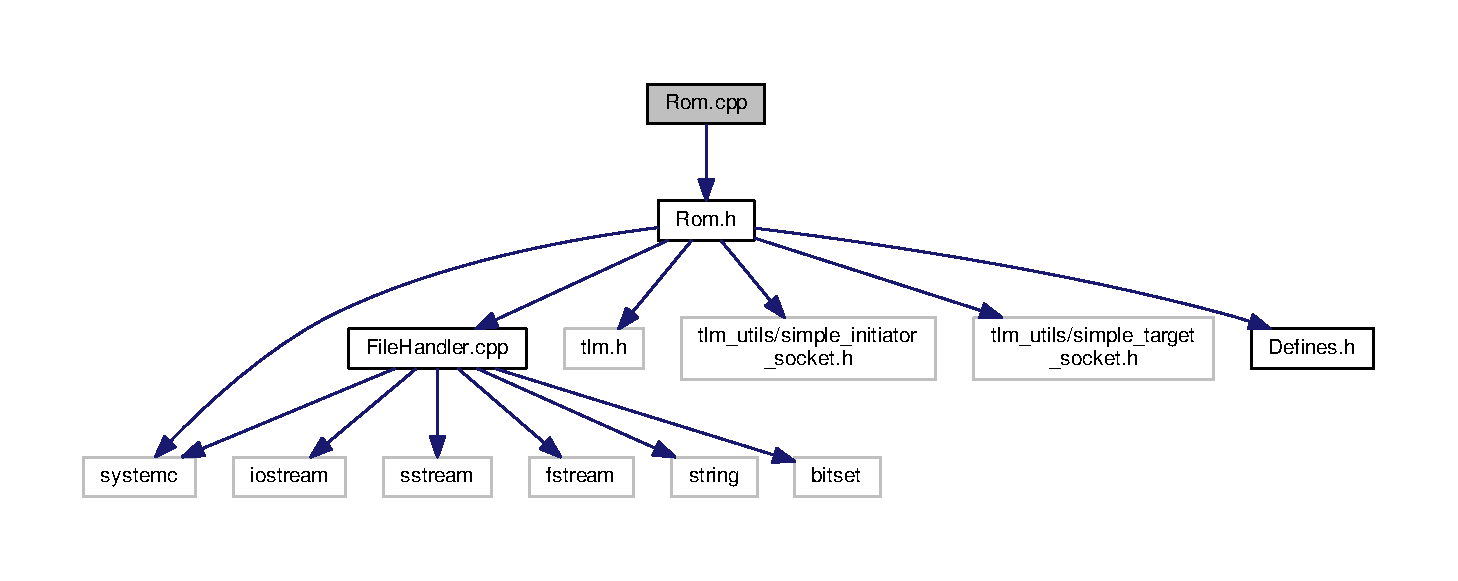
\includegraphics[width=350pt]{Rom_8cpp__incl}
\end{center}
\end{figure}

\hypertarget{Rom_8h}{\section{Rom.\+h File Reference}
\label{Rom_8h}\index{Rom.\+h@{Rom.\+h}}
}
{\ttfamily \#include \char`\"{}systemc\char`\"{}}\\*
{\ttfamily \#include \char`\"{}File\+Handler.\+cpp\char`\"{}}\\*
{\ttfamily \#include \char`\"{}tlm.\+h\char`\"{}}\\*
{\ttfamily \#include \char`\"{}tlm\+\_\+utils/simple\+\_\+initiator\+\_\+socket.\+h\char`\"{}}\\*
{\ttfamily \#include \char`\"{}tlm\+\_\+utils/simple\+\_\+target\+\_\+socket.\+h\char`\"{}}\\*
{\ttfamily \#include \char`\"{}Defines.\+h\char`\"{}}\\*
Include dependency graph for Rom.\+h\+:\nopagebreak
\begin{figure}[H]
\begin{center}
\leavevmode
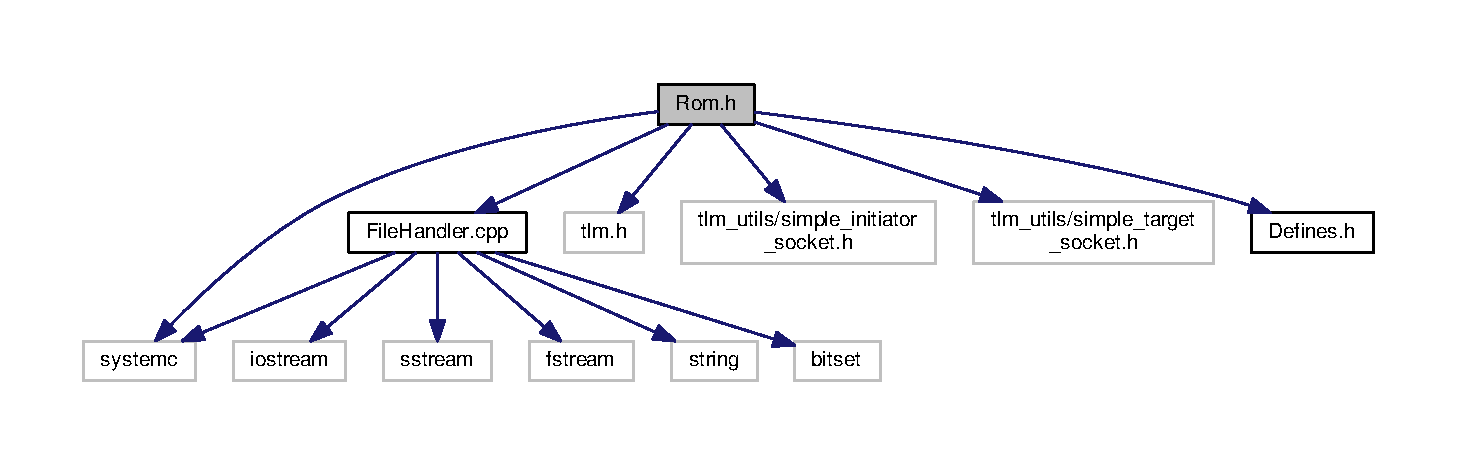
\includegraphics[width=350pt]{Rom_8h__incl}
\end{center}
\end{figure}
This graph shows which files directly or indirectly include this file\+:\nopagebreak
\begin{figure}[H]
\begin{center}
\leavevmode
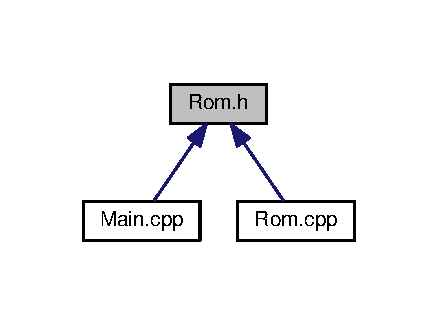
\includegraphics[width=210pt]{Rom_8h__dep__incl}
\end{center}
\end{figure}
\subsection*{Classes}
\begin{DoxyCompactItemize}
\item 
class \hyperlink{classRom}{Rom}
\begin{DoxyCompactList}\small\item\em Read-\/\+Only Memory. \end{DoxyCompactList}\end{DoxyCompactItemize}

\hypertarget{Stack_8cpp}{\section{Stack.\+cpp File Reference}
\label{Stack_8cpp}\index{Stack.\+cpp@{Stack.\+cpp}}
}
{\ttfamily \#include \char`\"{}Stack.\+h\char`\"{}}\\*
Include dependency graph for Stack.\+cpp\+:\nopagebreak
\begin{figure}[H]
\begin{center}
\leavevmode
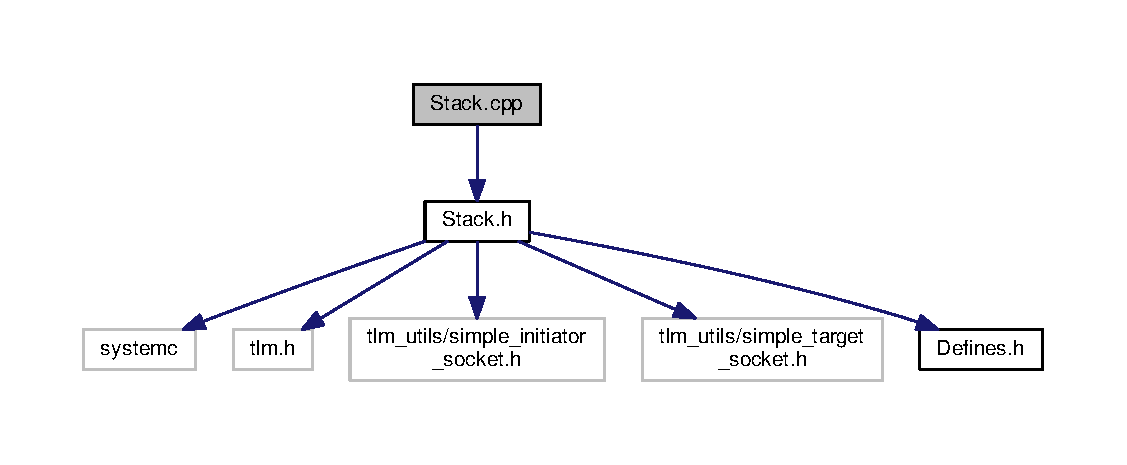
\includegraphics[width=350pt]{Stack_8cpp__incl}
\end{center}
\end{figure}

\hypertarget{Stack_8h}{\section{Stack.\+h File Reference}
\label{Stack_8h}\index{Stack.\+h@{Stack.\+h}}
}
{\ttfamily \#include \char`\"{}systemc\char`\"{}}\\*
{\ttfamily \#include \char`\"{}tlm.\+h\char`\"{}}\\*
{\ttfamily \#include \char`\"{}tlm\+\_\+utils/simple\+\_\+initiator\+\_\+socket.\+h\char`\"{}}\\*
{\ttfamily \#include \char`\"{}tlm\+\_\+utils/simple\+\_\+target\+\_\+socket.\+h\char`\"{}}\\*
{\ttfamily \#include \char`\"{}Defines.\+h\char`\"{}}\\*
Include dependency graph for Stack.\+h\+:\nopagebreak
\begin{figure}[H]
\begin{center}
\leavevmode
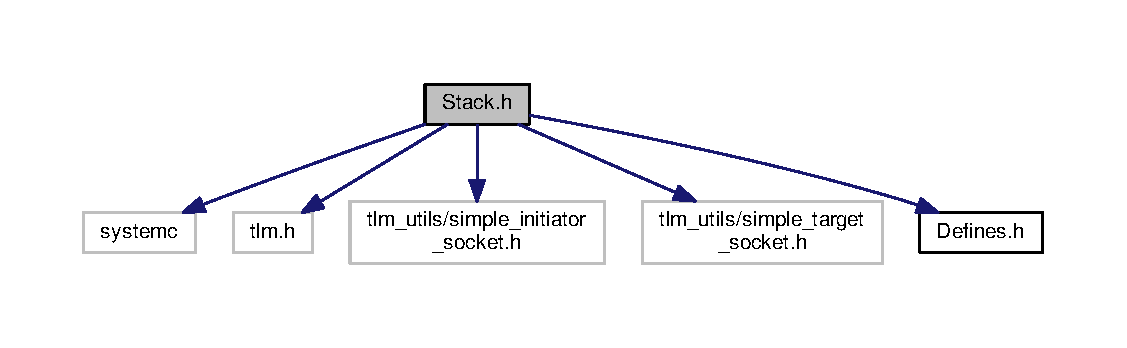
\includegraphics[width=350pt]{Stack_8h__incl}
\end{center}
\end{figure}
This graph shows which files directly or indirectly include this file\+:\nopagebreak
\begin{figure}[H]
\begin{center}
\leavevmode
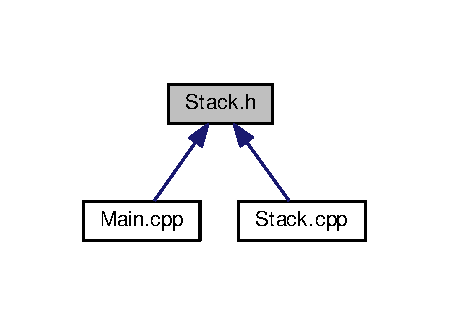
\includegraphics[width=216pt]{Stack_8h__dep__incl}
\end{center}
\end{figure}
\subsection*{Classes}
\begin{DoxyCompactItemize}
\item 
class \hyperlink{classStack}{Stack}
\begin{DoxyCompactList}\small\item\em Pilha de retorno. \end{DoxyCompactList}\end{DoxyCompactItemize}

%--- End generated contents ---

% Index
\newpage
\phantomsection
\addcontentsline{toc}{chapter}{Index}
\printindex

\end{document}
